\documentclass[12pt, a4paper]{book} %Esboco_Tese_Doutorado_2023-09-20
%\documentclass[tese]{abntex2} %Alternativa de tipo de documento (nesse caso, consultar documentação do pacote abntex2)
\usepackage[utf8]{inputenc} %Codificação
\usepackage[brazilian]{babel} %Idioma do documento e ortografia geral
\usepackage[alf]{abntex2cite}
\usepackage{epigraph} %Epígrafe
\usepackage{setspace} %Espaçamento de linhas
\usepackage{graphicx} %imagens
\usepackage[hycap]{caption} %legenda
    %\captionsetup[figure]{labelsep=none} %formato legenda
    \usepackage{chngcntr} %fazer contagem global das figuras
        \counterwithout{figure}{chapter} %fazer contagem global das figuras
\usepackage[colorlinks=true, allcolors=blue]{hyperref} %referência cruzada
    \renewcommand{\thefigure}{\arabic{figure}}
\usepackage{xcolor} %cor da fonte
    \definecolor{textcolor}{RGB}{56,74,103} %cor fonte livro Waldheim
    \definecolor{labelcolor}{RGB}{96,86,78} %cor legenda livro Waldheim
\usepackage{tcolorbox} %caixa de texto
%%%%%%%%%%%%%%%%%%%%%%%%%%%%%%%%%%%%%%%%%%%%%%%%%%%%%%%%%%%%%%%%%%%%%%%%%%
\begin{document}

\frontmatter % Seção de pré-texto (capa, sumário, resumo, etc.)

% Title Page
\title{Diretrizes Projetuais 

para Traçados Urbanos

Morfologicamente Adequados}

\author{Higor Ribeiro da Costa}
\date{Maringá, 2024}

    \maketitle

    \tableofcontents
    \listoffigures %Lista de figuras
    \listoftables %Lista de tabelas

    %\input{resumo} %Arquivo com o resumo da tese

    \mainmatter % Corpo principal da tese

    \onehalfspacing
    

    \part*{}

        \chapter*{Introdução}
        \addcontentsline{toc}{chapter}{Introdução}
        
        Há muito que me pergunto o porquê de nossas cidades serem tão `feias', e penso que isso tenha que ver com seus traçados. Talvez `feio' não seja o melhor termo para descrever esse aspecto da realidade, pois não se trata aqui de um mero juízo estético de minha parte. Porém, ``enquanto tem-se dificuldade para encontrar um parâmetro conjunto para o [termo] `belo', em relação ao [termo] `feio' parece ser menos problemático encontrar um terreno comum'' (Daverio, 2022, \textit{s.p.}, tradução nossa). `Se hoje temos tanta tecnologia, por que fazemos bairros e cidades assim?' Assim `desconjuntados', que `não fazem sentido.' Por que os loteamentos parecem `arranhões de gato' sobre as colinas, com ruas tão íngremes que não permitem a caminhada, dificultam o acesso do transporte, e promovem enxurradas que levam as casas para dentro dos rios? Essa foi uma dúvida que me perseguiu por anos, e, ao começar a entender as causas desse fenômeno, pesquisar uma solução – ou pelo menos uma alternativa – pareceu-me imprescindível.

        $<$FIGURA COM LOTEAMENTO DO TIPO `ARRANHÃO DE GATO'$>$

        É necessário salientar que entre o campo da edilícia e o da cidade há uma lacuna considerável. Quero dizer, quando falo em arquitetura `feia,' quero significar aquela arquitetura que não é orgânica – \textit{i.e.,} cujas partes não são interdependentes – e que não tem uma relação forte com seu contexto. E explicações para esse fenômeno não nos faltam (Caniggia e Maffei, 2008 [1979]; Strappa, 1995).

        Porém, para as cidades já não temos tantas explicações – talvez, precisamente, pela complexidade do tema. O que é uma cidade `feia'? É apenas uma cidade inorgânica? Uma cidade cujo traçado não tem relação com seu contexto – tanto natural como antrópico? E o que fez as cidades se tornarem assim? Mesmo quando a cidade `velha' tem uma certa beleza, o que faz com que as novas áreas urbanas tenham, não raro, uma qualidade inferior às antigas áreas urbanas? É certo que vemos as benesses das infraestruturas que não existiam no passado, no entanto, por exemplo, as áreas históricas de cidades antigas fazem os olhos de turistas – ainda que atraídos pelo marketing, mas um marketing que soube evidenciar as características positivas de tais áreas. E que características seriam essas? Posso apontar duas, pelo menos. A primeira é a coerência entre as edificações da área, não raro em um \textit{continuum} de fachadas que cria um grande cenário urbano – cenário autêntico. E a segunda é a conformação do traçado que lhes dá suporte – e isso é o que me interessa aqui.

        \begin{center}
        . . . . .
        \end{center}

        No fim de minha dissertação de mestrado, cheguei à conclusão de que é possível projetar traçados urbanos morfologicamente adequados ao contexto. E explico o que quero dizer com isso. `Contexto' aqui é o conjunto de estruturas naturais e antrópicas de uma área e suas respectivas características. `Morfologicamente adequado' quer dizer aquilo que já é, desde sua concepção, coerente com o formato das estruturas do contexto dado pela realidade. E traçado urbano é a marca das estruturas urbanas que o homem desenvolve.

        No caso das estruturas naturais, o que tomo por mais importante é a orografia, a terra com a sua forma, que é sobre onde se assentam as estruturas que o homem desenvolve, seguida pela hidrografia. Uma área pode ser mais íngreme ou suave, mais ou menos extensa, e seu relevo possui uma hierarquia latente, que pode ser destrinchada por meio de cumeadas e por talvegues. E, no caso das estruturas antrópicas, temos parcelamentos rurais precedentes, franjas urbanas com loteamentos, e diretrizes viárias. Com isso, temos ruas e avenidas, lotes urbanos e glebas rurais. Cada uma dessas estruturas naturais e antrópicas desenvolve uma relação de interdependência, existencial – pois algumas não podem existir sem outras – e morfológica, por meio de seus formatos poligonais e consequentes angulações – bidimensional ou tridimensionalmente. 

        Ou seja, quando digo que um traçado urbano deve ser `morfologicamente adequado ao contexto', quero implicar que cada um de seus elementos (sobretudo ruas, praças, demais espaços abertos, e os lotes e quarteirões que derivam de sua disposição) deve, na máxima medida possível, seguir, primeiro, os formatos dados pela estruturação natural e, segundo, os formatos dados pelos elementos da estruturação antrópica. E isso se opõe ao \textit{laissez-faire} dos traçados concebidos \textit{a priori} e só depois `adaptados' à realidade, que se impõe forçosamente ao projetista contrariado. Um traçado `adequado' é diferente de um traçado `adaptado'. É a morfogênese planejada contraposta ao automatismo.

        $<$FIGURA DE OUTDOOR COM ANÚNCIO DE LOTEAMENTO$>$

        \begin{center}
        . . . . .
        \end{center}

        Durante aquela pesquisa, da qual a presente tese não é senão o desdobramento, desenvolvi o conceito de `\textit{rendimento} urbano' – que afirma que deve existir uma ``coerência intrínseca'' entre o traçado urbano e o contexto natural (Costa e Rego, 2019, p. 7); e projetei um traçado urbano hipotético sobre uma área urbana consolidada, comparando-o com o traçado existente e com a legislação local em vigor. Com isso, verifiquei ser possível projetar traçados urbanos `de qualidade' (Costa, 2020, p. 106). Traçados com bom \textit{rendimento} urbano em termos ambientais, espaciais e econômicos.

        O que fiz na dissertação foi uma simulação baseada na síntese de um novo conceito (o \textit{rendimento} urbano) e em um estudo de caso (a partir do qual foram extraídos parâmetros para a avaliação desse conceito). Eu queria mostrar que um traçado urbano adequado ao sítio tinha lugar no mundo contemporâneo das cidades planejadas \textit{a priori}, posto que, hoje, um processo de desenvolvimento gradual da estrutura urbana, do traçado urbano, parece já não ter lugar – pois o \textit{status quo}, hoje, é o da morfogênese substituída pelo `mecanicismo'. 

        Outrora, as ruas não eram senão a afirmação de percursos pré-existentes, sulcados ao longo do tempo no relevo do território por inúmeras gerações que nos precederam (Caniggia e Maffei, 2008).   Esses percursos, primitivamente utilizados apenas como rotas de passagem, passaram a ser a estrutura de acesso a áreas inicialmente de caça e coleta, posteriormente de cultivo, até chegar à sua partição em propriedades. E, nos locais mais propícios, tais percursos tiveram seus formatos consolidados, consagrados na matéria, por meio das fachadas das edificações que os margeavam. Era a formação do que, no universo lusófono, chamamos de ``rua", com a série de edificações a ela rentes.

        Observando esse processo, não é difícil perceber que eram os saberes tradicionais da consciência espontânea e a acomodação ao legado das gerações anteriores que capitaneavam a formação de ruas – ou melhor, de `percursos edilícios'. E o direito consuetudinário os mantinha com suas características. Hoje, porém, temos leis positivistas que ditam de antemão como um projeto pode ser feito – seja um arruamento, um parcelamento ou um \textit{masterplan}. E é esse projeto que vai moldar a realidade material que constituir-se-á em um sítio. É toda uma outra dinâmica. Assim, naquele momento decidi projetar um novo traçado urbano adequado às exigências da contemporaneidade, porém projetado a partir de um esquema `à antiga'.



        Noto a existência de traçados urbanos adequados à topografia do sítio e de traçados feitos à revelia do relevo – estes últimos relacionados a diversos problemas, sendo oriundos daquilo que chamo `\textit{modus faciendi} atual' (Costa \textit{et al.,} 2020). Pude perceber isso em diversas cidades, e não foi diferente com Maringá-PR, meu local de estudo e experimentação até o momento. Nela, o traçado do plano original da cidade – projetado por Jorge de Macedo Vieira – se encaixa na primeira categoria, e o traçado das expansões urbanas – desenvolvido sobre o parcelamento rural da Companhia – na última.  

        $<$INSERIR IMAGEM$>$

        O primeiro grupo congrega traçados urbanos orgânicos, com elementos interdependentes que, em geral, não são serializáveis ou intercambiáveis. Tais traçados podem ser oriundos tanto de um desenvolvimento espontâneo como de um processo de planejamento. E, em ambos os casos, o que se vê é um processo de formação ou desenvolvimento projetual mais complexo e elaborado, e, consequentemente, mais prolongado no tempo, adequando-se de modo particular às características físicas do sítio. 

        Já o segundo grupo congrega traçados não-orgânicos e intercambiáveis, oriundos do \textit{modus faciendi} atual. Neles, é possível observar uma lógica `mecanicista' subjacente, na qual prioriza-se um retorno financeiro ligado à venda de lotes, dispostos geralmente em quadras ortogonais.

        O resultado da aplicação indiscriminada de traçados abstratos, de concepção alheia ao contexto no \textit{modus faciendi} atual são ``territórios descontínuos e paisagens contraditórias'' (Strappa, 2018, p. 11, tradução nossa). Loteamentos e loteamentos que `brotam' como fungos a partir das cidades, de suas franjas e conexões.
            \footnote[4]{A expressão `fungos' foi utilizada pelo professor Philippe Daverio (2018). Empreendimentos urbanos (\textit{i.e.,} loteamentos) em locais inusitados, conectados às áreas urbanas consolidadas apenas por meio de uma pequena estrada, assim como os fungos também se reproduzem e espalham `em rede'. Portanto, a analogia permanece válida.} 
        Geram-se, assim, manchas urbanas formadas por traçados desconexos entre si. E o que se percebe é uma tendência à segregação dessas novas áreas urbanas, bem como uma diminuição da mobilidade, com a sobrecarga das poucas vias de acesso – em geral íngremes.

        Além disso, não há uma distinção clara ou uma integração sustentável entre a mancha urbana e o território natural. Diversas ruas fazem `incursões' em áreas que, por sua morfologia e características naturais, deveriam ser preservadas. E, desse modo, o que ocorre não é uma integração entre a cidade e o campo, ou o dissolver das estruturas urbanas no território circunstante, mas sim uma espécie de `corrupção' de todos: cidade, campo e natureza.



        Para projetar o novo traçado urbano `à antiga' ao qual me referi antes, lancei mão de um estudo de caso, fazendo uma leitura morfológica do traçado original projetado para a cidade de Maringá-PR, reputado como uma solução moderna e adequada às pré-existências do sítio – concomitantemente com o parcelamento rural da companhia colonizadora (CTNP/CMNP) que encomendou o projeto (Rego, 2009, 2001; Rego \textit{et al.}, 2004; Bonfato, 2008; Beloto, 2015; Meneguetti, 2007; Kohlhepp, 2015; Waibel, 1949). A partir do traçado original de Maringá, extraí parâmetros de avaliação do \textit{rendimento} urbano que poderiam ser aplicados na conformação de novos traçados urbanos. E, para provar que os era possível utilizar, projetei um novo traçado urbano sobre uma área da atual cidade de Maringá – uma expansão urbana fora dos limites do plano original da cidade, e com uma `qualidade' inferior a este. Feito isso, desenvolvi um estudo comparativo quantitativo entre os dois traçados urbanos e a legislação atual (\autoref{fig:comparativo_tracados}), verificando ser possível projetar um traçado urbano adequado ao sítio com uma `qualidade' superior ao \textit{modus faciendi} atual e mantendo índices semelhantes, desde que aplicando o conceito de \textit{rendimento}.

        \begin{figure}[h]
            \centering
            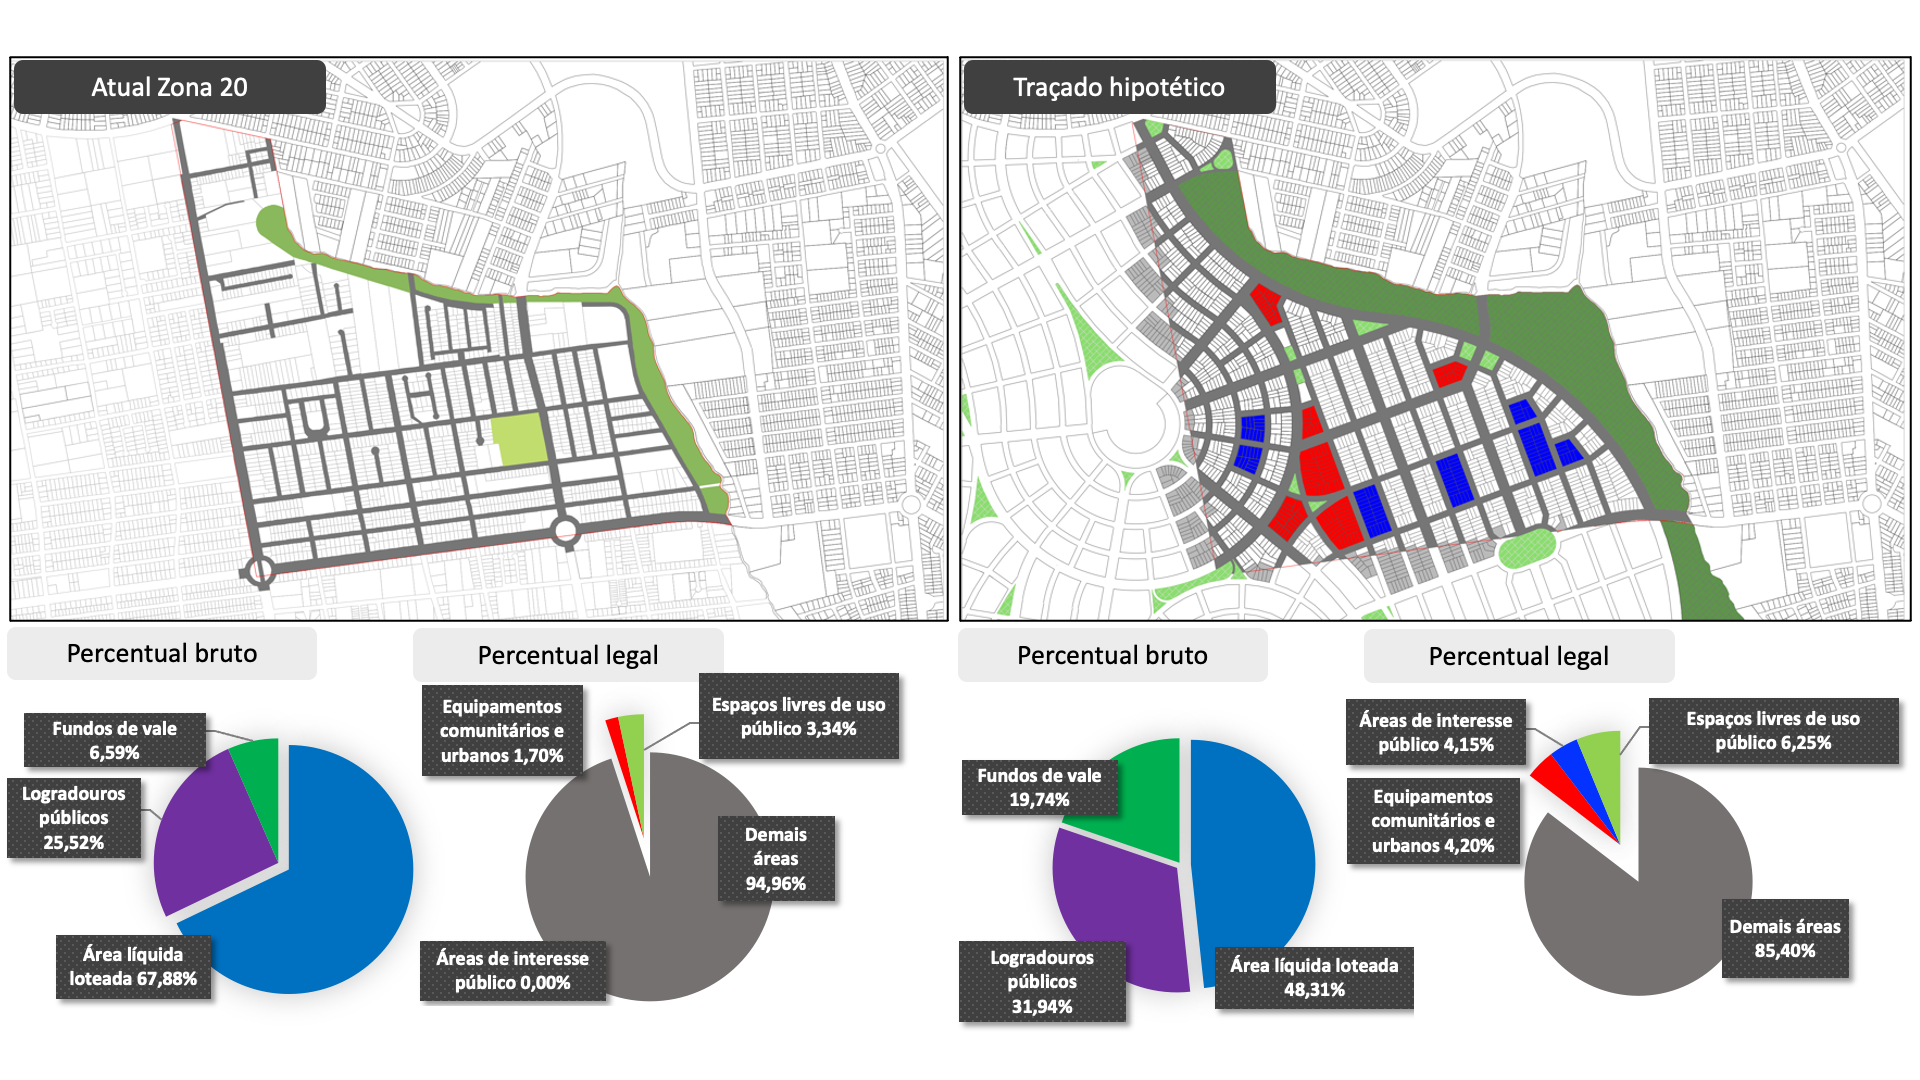
\includegraphics[width=1\textwidth]{/Users/Pancratii/GitHub/phd/Sections/Projeto_de_Pesquisa_2023-03-18_Teste/Pictures/comparativo_tracados.png}
            \captionsetup{labelfont=bf}
            \caption{Comparativo entre o traçado existente (à esquerda) e o traçado hipotético projetado (à direita). \textbf{Fonte:} Costa, 2020 (adaptado).}
            \label{fig:comparativo_tracados}
        \end{figure} 

        \begin{center}
        . . . . .
        \end{center}

        

        \begin{center}
        . . . . . 
        \end{center}


        Uma justificativa razoável para a presente empresa é a ausência de estudos prescritivos para traçados urbanos sob a luz da coerência entre traçado e contexto. No campo da morfologia urbana, existem estudos de observação e análise de traçados urbanos, como a metodologia \textit{Morpho} (Oliveira e Silva, 2013; Oliveira e Medeiros, 2016), mas que não consideram a topografia; ou estudos que consideram as formas do terreno no território e outros fatores ligados à sustentabilidade ambiental (Fanta \textit{et al.,} 2022), mas que não adentram no tocante específico dos traçados urbanos e de seus formatos. Ambos de caráter não-prescritivo. Neles, vê-se a ausência de diretrizes prescritivas para o desenho das cidades, sobretudo diretrizes que agreguem \textit{savoir-faire} de diferentes áreas do conhecimento. Até existem manuais de projeto, porém, ou eles datam de mais de um século, como é o caso de Unwin (1909) e Sitte (1889), ou, mais recentemente, tratam mais de aspectos relacionados ao `aproveitamento' e infraestruturas de loteamentos, como é o caso de Mascaró (2003); e, em ambas as situações, pouco ou nada se fala do aspecto ambiental do traçado urbano. Mais recentemente, até surgem novos manuais, porém, mais voltados ao desenho urbano na escala da rua do que na escala do traçado: canteiros, mobiliário, distribuição das faixas e arborização são seus objetos, não a morfologia urbana em escala mais ampla (Del Rio, 1999; Carmona \textit{et al.,} 2003; Carmona e Sieh, 2004; Carmona e Steven, 2007; Steiner e Butler, 2007; Caniggia e Maffei, 2008). Há diretrizes, e até métodos para a análise que dá suporte a um possível processo de projeto, mas não uma prescrição endereçada diretamente a tal (Oliveira, 2016, 2018; Doherty e Waldheim, 2016; Waldheim, 2016). Há ainda o método de projeto desenvolvido no âmbito dos workshops W.A.M. (Maretto, 2018), e aquele presente no trabalho de Saverio Muratori para o programa habitacional INA-Casa (Maretto, Costa e Rego, 2023) – ambos prescritivos. Porém, em ambos, ainda que havendo alguma consideração pela topografia (sobretudo no exemplo muratoriano), parte-se de uma realidade edificada pré-existente, com tecidos urbanos históricos, ou em áreas novas (ou de intervenção) nas bordas de uma realidade construída já consolidada. E isso sem falar que aqui tratamos de projetos \textit{à la masterplan}, ou seja, de um processo que depende do arquiteto e de um ente que possa levar a cabo toda a empreitada, diferente do processo de formação da cidade, com seus diferentes atores e fontes de receita (Alexander \textit{et al.,} 2013).

        É verdade que, sobretudo na primeira metade do século XX, houve iniciativas a tentar sanar essa situação problemática que aponto nas expansões urbanas. Estas iniciativas tratavam a cidade como habitat humano que deveria ser melhorado: estética, logística e funcionalmente. E isso por meio da relação cidade-campo, da densidade (Howard, 1902), de determinados arranjos formais do traçado (Unwin, 1909; Sitte, 1992) ou da dissolução da cidade tradicional em favor de utopias (Le Corbusier e Etchells, 1987; Le Corbusier, 1991). Enquanto isso, nos últimos 50 anos, viu-se um emergir de considerações ambientais (McHarg, 1971), não mais da cidade, mas da `paisagem' (Doherty e Waldheim, 2016).\footnote[5]{As definições de `paisagem', \textit{`landscape'} e \textit{`paesaggio'} serão destrinchadas no momento oportuno.} E, mais recentemente, podemos ver a ideia de \textit{`landscape'} enquanto \textit{`framework'} das cidades e regiões dentro do chamado \textit{`landscape urbanism'} (Waldheim, 2016). No entanto, em nenhum desses casos é possível identificar um estudo metódico do processo de morfogênese. Isso só se fez mais visível no arcabouço teórico-metodológico da escola italiana de tipomorfologia urbana – pouco conhecida e divulgada, precisamente por ser uma `escola', e não um `ideário' com princípios a aplicar por toda parte. E ainda assim, a escola italiana trata de leitura e análise urbano-territorial com ênfase projetual na escala das edificações, ou em projetos urbanos (\textit{`masterplan'}). Ou seja, ou oito, ou oitenta.
   
        Desse modo, faltam diretrizes claras para projetar traçados de maneira coerente e orgânica, e que possam ser considerados adequados e belos. E é diante desse problema que me pergunto: `como projetar um traçado urbano morfologicamente adequado ao contexto?' 

        Com esta tese, o que pretendo é desenvolver um conjunto de diretrizes que possam ser aplicadas em diferentes contextos. E meu intuito com isso é gerar uma alternativa ao \textit{modus faciendi} atual. Para isso, eu preciso ampliar o horizonte do conceito de \textit{rendimento} para além do traçado urbano enquanto algo estanque, tornando-o aplicável na dinâmica da realidade. Ou seja, devo relacionar o conceito de \textit{rendimento} urbano com o processo de expansão urbana e com as estruturas naturais e antrópicas que lhe servem de \textit{framework} – nesse caso, expansões extra-urbanas, peri-urbanas e/ou intra-urbanas. E, a partir disso, desenvolver um artefato (conjunto de diretrizes) que possa ser utilizado por todos aqueles que projetam traçados, e, com isso, produzem cidades e territórios, tais como projetistas, empreendedores, imobiliaristas, legisladores, gestores, pesquisadores, docentes, alunos como `alternativa' ao modo de fazer traçados urbanos hoje em voga.

        \begin{center}
        . . . . .
        \end{center}

        Ademais, se é verdade que consegui projetar um traçado urbano adequado a um determinado contexto, não necessariamente é verdade que uma outra pessoa o conseguirá fazer em outro contexto. Faz-se mister pôr à prova o estratagema que utilizei. E como tornar isso palpável? Por meio de um software ou algoritmo, no qual fosse necessario fornecer apenas algumas instruções, dar um \textit{input}? Bom, nesse caso eu precisaria de uma equipe, e diretrizes já delineadas e organizadas metodicamente, coisa que é inviável no prazo de quatro anos de um doutorado – ao menos para um leigo em linguagem de programação. Então por meio de um método, com um passo-a-passo? Não necessariamente, posto que isso engessaria a aplicação do projeto quando em diferentes contextos e circunstâncias. Bem, nesse caso, por exclusão, cheguei à determinação de que são necessárias diretrizes de projeto, um conjunto de diretrizes para o processo de projetar traçados urbanos morfologicamente adequados ao contexto. 

        %Método
        Para desenvolver tais diretrizes, lanço mão da \textit{Design Science Research} (DSR) como método de pesquisa (Dresch \textit{et al.,} 2013; Lacerda \textit{et al.,} 2015), por ser um método prescritivo que visa a melhoria de processos já existentes. No caso em questão, prescritivas são as diretrizes de projeto, e a realidade ou processo existente a ser melhorado é o processo de projeto de traçados urbanos.

        Fulcrais na DSR são: o desenvolvimento de um `artefato' (aqui, o conjunto de diretrizes), e a avaliação e comunicação dos resultados por e para os \textit{stakeholders} (que, no caso em questão, são profissionais, gestores, pesquisadores, docentes e estudantes que lidam com o processo de projeto de traçados urbanos). Tal método de pesquisa é constituído por fases, sendo elas: (1) consciência do problema; (2) sugestão; (3) desenvolvimento; (4) avaliação; e (5) conclusão. Tais fases se retroalimentam entre si, e seus produtos são: (a) proposta; (b) esboço; (c) artefato; (d) mensuração; e (e) resultados (Vaishnavi e Kuechler, 2021 [2004]).

        %[17NOV2023 19:56 UEM] 
        Na primeira etapa desse método, deve-se ``identificar e compreender o problema que [se] deseja estudar e solucionar'', bem como ``definir qual é a \textit{performance} necessária para o sistema em estudo'' – performance essa que será medida posteriormente (nas etapas de desenvolvimento e avaliação) com parâmetros extraídos da revisão de literatura e de um estudo de caso. Na segunda etapa, são sugeridas possíveis soluções para o problema de maneira abdutiva – nesse caso, por meio da definição de três situações para traçados hipotéticos. Na terceira etapa, ocorre o desenvolvimento de um dos artefatos propostos na segunda etapa – ou seja, um conjunto de diretrizes que serão extraídas a partir do projeto desses traçados hipotéticos. As diretrizes que se mostrarem adequadas na solução do problema (relativo ao processo de projeto de traçados morfologicamente adequados) serão avaliadas em uma quarta etapa (Dresch \textit{et al.}, 2015, p. 79; Vaishnavi e Kuechler, 2021, pp. 11-13). E é essa disposição das etapas que se desdobra na formatação dos capítulos desta tese.

        Na presente pesquisa, associo a DSR com estratégias como estudo de caso, modelagem, simulação e grupo focal, de modo a compreender a realidade na qual pretendo intervir, identificar diferentes possibilidades dentro da realidade em questão, desenvolver um arcabouço de soluções, e verificar se tais soluções são aplicáveis em outras realidades.

        Assim, para preencher tal lacuna e alcançar o objetivo acima proposto, na senda da \textit{Design Science Research}, fazem-se necessárias as seguintes etapas, que se refletem no delineamento da pesquisa: 
            \begin{itemize}
                \item Revisar conceitos e métodos tanto atinentes ao processo de projeto de traçados urbanos como à morfologia urbana, particulamente àqueles afins ao conceito de \textit{rendimento}; 
                \item Buscar soluções semelhantes que já tenham sido aplicadas (como \textit{guidelines, patterns,} métodos, leis, manuais, livros) na classe de problema em questão (\textit{i.e.,} ausência de método de projeto), além de selecionar e esboçar um tipo de solução a ser desenvolvida;
                \item Efetuar um estudo de caso sobre Maringá, com levantamento documental e cartográfico, leitura morfológica e revisão de literatura acerca do projeto original, das expansões urbanas, do parcelamento rural e das diretrizes viárias, bem como revisão da legislação atual; %e entrevistas com \textit{stakeholders} para entender as premissas, motivações e o processo de projeto no \textit{modus faciendi} atual; 
                \item Estabelecer um protocolo para o desenvolvimento do conjunto de diretrizes; 
                \item Desenvolver um conjunto de diretrizes piloto por meio de modelagem e simulação (com traçados urbanos hipotéticos); 
                \item Avaliar o conjunto de diretrizes por meio de comparativo com legislação, situação, morfologia e \textit{modus faciendi} atuais (para aferir viabilidade), e por meio de um grupo focal (para avaliar aplicabilidade em outros contextos); e, por fim,
                \item Refinar e sintetizar as diretrizes do conjunto.
            \end{itemize}

        \begin{center}
        . . . . .
        \end{center}

            \section*{Estrutura da Tese}

            A presente tese está estruturada em cinco capítulos, dispostos em três partes. A primeira parte da tese – intitulada `consciência' – é composta pelo primeiro e segundo capítulos. No primeiro capítulo é feita a revisão de literatura, de modo a formular um marco teórico-conceitual para a tese. E no segundo capítulo um estudo de caso é realizado sobre Maringá, com levantamento documental e cartográfico, leitura morfológica e revisão de literatura acerca do projeto original, das expansões urbanas, do parcelamento rural e das diretrizes viárias, bem como revisão da legislação atual.

            Já a segunda parte da tese – chamada `desenvolvimento' – abrange o terceiro capítulo. Aqui, apresento três pilotos, projetos hipotéticos de traçados urbanos. O primeiro foi desenvolvido durante o mestrado, sozinho, sobre um promontório inteiro, ou seja, uma espécie de \textit{tabula rasa} e um piloto inicial de traçado urbano. O segundo traçado foi desenvolvido durante enquanto orientei um projeto de iniciação científica, considerando algumas pré-existências antrópicas da área estudada, como diretrizes viárias, avenidas e faixas de domínio pré-existentes; portanto, um piloto de desenvolvimento semi-autônomo das diretrizes por parte de \textit{stakeholders} (eu e o aluno orientado), ao mesmo tempo que abarcando áreas intra-urbanas, o que indica a possibilidade de uso das diretrizes em áreas urbanas sub-utilizadas, ou na pesquisa e no estudo comparativo (acadêmico) de possíveis alternativas ao modo como atualmente se projetam traçados urbanos. E o terceiro foi desenvolvido no âmbito desta tese, considerando um processo de expansão urbana cujos módulos são os lotes rurais paulatinamente ocupados por loteamentos estruturados por uma estrutura comum (eventualmente um \textit{framework}). Neste capítulo, assim, são apresentados tais traçados e o passo-a-passo de seu desenvolvimento projetual, levando a diretrizes preliminares de projeto.

            Por fim, a terceira parte da tese – `avaliação' – contempla a verificação das diretrizes preliminares de projeto por meio do penúltimo capítulo (com o comparativo entre os resultados obtidos nas simulações e a realidade existente, e por meio de um grupo focal, que deve testar as diretrizes preliminares em diversos contextos país afora). E, no último capítulo, elenca de maneira sistematizada as diretrizes de projeto destiladas e testadas no decorrer da tese como um todo.


    
    \part[Consciência]{Consciência}

        \chapter[Revisão de literatura: projeto, traçado, morfologia e desenho urbanos]{Revisão de literatura: projeto, traçado, morfologia e desenho urbanos}

        \epigraph{``We need to think of the street, the district, the town as larger wholes, and find a glorious function and a worthy guidance for the decorative treatment of each plot and each house in so designing them that they shall contribute to some total effect. \textit{For is it not a finer thing to be a part of a great whole than to be merely a showy unit among a multitude of other units?}}{Unwin, 1909, p. 288, destaques nossos.}

        Precisamos pensar a rua, o bairro, a cidade como conjuntos. Cada um deles deve colaborar com o todo. A ideia não é minha, mas de Sir Raymond Unwin (1909, p. 288). Esse princípio – da subordinação das partes ao todo – é o mesmo que rege o \textit{``rendimento''} em sua concepção original, de que tratei em minha dissertação de mestrado (Costa, 2020). Um traçado morfologicamente adequado, assim como proposto nesta tese, é um traçado com \textit{``rendimento''}.
        
        No âmbito da escola italiana de tipomorfologia, \textit{``rendimento''} é ``a dialética entre uma ação antrópica e uma reação ambiental, constituída pelo menor ou maior esforço com que o ambiente tenderá a reabsorver o resultado daquela ação'' (Caniggia e Maffei, 2008, p. 52, tradução nossa). Ação que é basicamente a intervenção feita por um indivíduo ou grupo durante um intervalo de tempo. Ambiente que é um conjunto unitário, resultante de diversas intervenções feitas ao longo do tempo, como um amálgama. E reação que é basicamente `o que ocorre depois que a ação é feita', um desencadear de novas ações que modifica o ambiente a partir dessa ação `inicial'. Quanto maior o \textit{rendimento} de uma intervenção, menor o esforço do ambiente para absorvêla e ``torna-la coerente com seu contexto'' (Rebecchini, 2008, p. 107, tradução nossa). Desse modo, o \textit{rendimento} diz respeito a uma relação de equilíbrio entre cada ação (parte) com o ambiente (o todo), sendo a dialética entre algo novo e um universo já existente. Ou seja, em princípio, o \textit{rendimento} pode ser entendido como ``grau de coerência com o contexto'' (Maffei, 2003, p. 82, tradução nossa).

        Este conceito de \textit{rendimento} tem sido aplicado apenas na escala da edificação – \textit{rendimento} edilício (Caniggia e Maffei, 2008; Caniggia, 1963; Cataldi, 2015; De Martin, 2009; Rebecchini, 2008; Dalla Negra, 2015; Marzot, 2015) – e na escala do território – \textit{rendimento} territorial (Carlotti, 2015). Não havia ainda a aplicação desse conceito na escala da cidade, tanto menos em língua portuguesa. E o resultado da pesquisa redundou no ``rendimento urbano'' ser concebido como ``a coerência intrínseca entre o traçado da forma urbana e o contexto natural'' (Costa e Rego, 2019, p. 7).

        Para entender o traçado da cidade e o que fazer com ele, proponho duas revisões de literatura. A primeira é uma revisão assistemática, com os principais autores relacionados ao projeto de traçados urbanos e ao estudo da forma urbana, de modo a verificar que parâmetros são divisados por esses autores como qualidades e parâmetros balizadores de projeto. A segunda é uma revisão sistemática de literatura para identificar manuais e \textit{guidelines} contendo diretrizes de projeto, no Brasil e no exterior.

        Os autores utilizados na revisão assistemática de literatura são: Raymond Unwin (1909), Camillo Sitte (1992), Vicente del Rio (1999), Juan Luís Mascaró (2003), Matthew Carmona \textit{et al.} (2003), Matthew Carmona e Louie Sieh (2004), Matthew Carmona e Tiesdell Steven (2007), Frederick Steiner e Kent Butler (2007), Gianfranco Caniggia e Gian Luigi Maffei (2008), Álvaro Rodriguez (2010), Spiro Kostof (2014), Gerd Wilhelm Kohlhepp (2015), Staël de Alvarenga Pereira Costa e Maria Manoela Gimmler Netto (2015), Vitor Oliveira (2016, 2018), Charles Waldheim (2016), Gareth Doherty e Charles Waldheim (2016), Huimin Ji e Wowo Ding (2021), e Václav Fanta \textit{et al.} (2022).

            %\begin{itemize} %Livros para leitura (ver quais parâmetros que eles dão como qualidade e que devem ser levados em conta no momento de projetar um traçado urbano)
              %  \item Unwin
                %\item Sitte
                %\item Mascaró %(para tratar do modus faciendi atual, de como se ensina ou o que se consulta na hora de projetar traçados)
                %\item Del Rio
                %\item Kostof
                %\item Vitor Oliveira
                %\item Caniggia e Maffei
                %\item Álvaro Rodriguez
                %\item Waldheim (os dois livros)
                %\item Kohlhepp
                %\item Fanta et al.
                %\item Legislação (brasileira e local) %Levar em conta que isso pode variar no caso de outros países
                %\item Carmona
                %\item Manual de urbanismo (Gislaine)
            %\end{itemize}
                
        Unwin (1909) por conta da vinculação de Jorge de Macedo Vieira com a sua prática projetual, e por ser um dos clássicos da literatura de projeto, mas que, diferente de outros autores, não foi traduzido para o português. Sitte (1992) porque Unwin é tributário de Camillo Sitte. Mascaró (2003) e Del Rio (1999) para entender o que é levado em conta no Brasil no momento de projetar traçados, sendo utilizado nos currículos das universidades brasileiras. Wo e Ding (2021) para definir o conceito de traçado urbano empregado nesta tese. Costa e Netto por sua sistematização e exemplos do emprego de metodologias de diferentes escolas de morfologia urbana. Vitor Oliveira (2016, 2018) por suas recentes descobertas no campo da morfologia urbana e sua aplicação no projeto de traçados urbanos. Caniggia e Maffei (2008) por trazerem à baila o modo como as cidades se estruturam organicamente. Álvaro Rodriguez (2010) e Charles Waldheim (2016) por conta da evolução do processo de urbanização e da atual relação entre o território e a cidade – e, por consequência, seu traçado. Em seguida, Kohlhepp (2015) e Fanta \textit{et al.} (2022), para entender o tipo de parcelamento rural do território de Maringá, sobre o qual novos traçados urbanos vêm sendo projetados. E, por fim, a legislação, de modo a ter um panorama daquilo que pode ser aplicado na prática no local utilizado para estudo.
   

        \begin{center}
        . . . . .
        \end{center} 

            %Mascaró, p. 13
            ``Todo sítio tem na topografia suas caracteristicas principais.'' A frase não é minha, mas de Juan Luis Mascaró (2003, p. 13), autor de um dos mais conhecidos manuais de ``Loteamentos Urbanos''.

            \begin{quotation} 
                \textit{Obviamente, nas declividades, na uniformidade, no tamanho dos morros e das bacias e em outros aspectos do relevo estarão os mais fortes condicionantes do traçado urbano.
                Igualmente, cada sitio tem seu ecossistema natural que, em maior ou menor grau, e alterado e agredido quando sobre ele se faz um assentamento urbano. O novo sistema ecologico criado podera ser agradavel ou não, estável ou instável, econômico ou antieconômico, dependendo, em grande parte, do critério com que o urbanista o trata.
                Não se pode dar uma regra geral, mas geralmente os sistemas mais agradáveis são aqueles que contém menores alterações, tornando-se mais econômicos e estáveis no tempo.
                Com os modernos equipamentos de grande capacidade para os movimentos de terra que tanto orguIham os técnicos dessa area tem-se condições técnicas de criar sítios com topografia totalmente artificial. Frequentemente se vê áreas de relevo complexo serem aterradas e desbastadas completamente, para ali ser criado um perfil topográfico mais simples, objetivando facilitar a subdivisão e a posterior edificação das residencias. Mais simples, sim; melhores, não. 
                Os assentamentos humanos que geralmente mais agradam são aqueles que parecem ter se desenvolvido de forma espontânea, aqueles lugarejos que aparecem como encravados na propria natureza. Curiosamente, esse tipo de assentamento que respeita a natureza é mais economico para implantar, porque dispensa os grandes movimentos de terra. Também se torna mais econômico de manter, porque é ecologicamente mais estável. 
                [E] Visto dessa outra perspectiva, evidencia-se que o desenho urbano não pode ser feito resolvendo apenas o problema na planta. Para se obter um bom desenho, deve-se trabalhar em suas três dimensões, levando em consideração que as soluções escolhidas necessitam se adaptar e serem oriundas das condições topográficas. 
                Embora isso seja muito claro, é frequente encontrar nos compêndios de desenho urbano diferentes traçados alternativos, colocados como se fossem de livre escolha, como se nada tivessem a ver com a topografia.}
            \end{quotation}

        \begin{center}
            . . . . .
        \end{center} 

        \chapter[Maringá, um estudo de caso]{Maringá, um estudo de caso}

        Para propor diretrizes projetuais para traçados urbanos morfologicamente adequados, é necessário ter um ponto de partida: algum exemplo real do qual extrair pontos que podem ser aplicados em outras situações, diatópica e diacronicamente, alcançando um resultado igualmente `bom', ainda que seu formato não seja necessariamente semelhante. Nesse sentido, penso que posso tomar a cidade de Maringá, no norte do Paraná, como esse exemplo. Não apenas por ser uma cidade à qual tenho acesso, por nela habitar, e por já ter me debruçado nela durante a dissertação de mestrado – o que me dá um melhor conhecimento sobre a mesma –, mas, sobretudo, pelo relato de diversos autores, que a reputam como sendo uma cidade que apresenta uma formação e traçado ímpares, desde a escolha do sítio de implantação até a disposição dos percursos, parcelamentos, edificações e espaços livres. Assim, desse ponto de vista, a leitura morfológica do traçado inicial de Maringá, feita a partir da análise da obra seminal de Raymond Unwin – que, direta ou indiretamente, norteou o projeto de Maringá – possibilita a identificação de parâmetros que nortearão novos traçados hipotéticos, dos quais extrair diretrizes projetuais.

            \section{Town Planning in Practice, Sir Raymond Unwin}
        
        Raymond Unwin, em seu tratado ``Town Planning in Practice: an introduction to the art of designing cities and suburbs'' (1909), expõe em detalhe diversos casos, os quais analisa e dos quais toma exemplo para diretrizes de projeto. Unwin divide sua obra em 12 capítulos, tratando sobre \textit{``Town planning''} e \textit{``Site planning''}, em duas escalas distintas, ainda que, segundo o autor, sem uma linha de demarcação. No \textit{``town planning''}, ``a primeira consideração deve ser a conveniência geral da cidade e o arranjo das principais vias''. Enquanto isso, no \textit{``site planning''}, a consideração recai no ``arranjo das edificações e no desenvolvimento do local" (Unwin, 1909, p. 289, tradução nossa). Desse modo, minha atenção recai sobre o \textit{``town planning''}.

        O manual de projeto de Unwin se inicia afirmando que é necessário classificar as cidades com diferentes tipos de traçado: aqueles ``que evoluíram por meio do crescimento natural'' e aquelas cidades ``que foram projetadas em diferentes períodos'' (Unwin, 1909, p. 16, tradução nossa). E, enquanto no mundo clássico, muito se vê de ângulos retos indo de Norte a Sul (pp. 45-46), nas cidades medievais as irregularidades parecem ter um planejamento, diferente do que estamos acostumados a pensar. Um planejamento feito no nível do transeunte, no olho (p. 52).\footnote[4]{Essa observação é importante, pois perpassará toda a obra de Unwin.}

        Em um passado mais recente, durante a Renascença, nos séculos XVI e XVII, o renascimento das artes e estudos clássicos teve um papel decisivo no planejamento das cidades, pois ``a Renascença trouxe consigo o poder e a coragem para lidar com o planejamento em larga escala e desenvolveu o que se pode chamar de uma grande abordagem em esquemas de organização'' (Unwin, 1909, p. 69, tradução nossa). E, nesse ínterim, a fundação de novas cidades tornou-se a ocupação favorita de diversos príncipes, desenhando-as com as linhas retas e formais típicas da Renascença.

        Para Unwin (p. 84), o que se desenvolveu foi uma verdadeira escola de planejadores renascentistas, cujas obras (traçados) eram desenvolvidas em grandes propriedades, com linhas rígidas e formais. E isso perdurou – ao menos na Europa – até o despontar da escola de paisagismo. O resultado disso foi que as cidades cresceram de modo caótico, com cada proprietário ``desenvolvendo sua própria terra sobre linhas que atentiam aos seus interesses ou caprichos'', resultando em traçados que deveriam prover ``o máximo número de locais para construção com o menor custo'' (Unwin, 1909, p. 88, tradução nossa).

        Por outro lado, porém, surgia uma outra escola de planejamento urbano, baseada nas conclusões de Camillo Sitte de que as cidades medievais eram, sim, planejadas. Não planejadas para o tráfego, mas sim de acordo com princípios artísticos (Unwin, 1909, p. 98). E, para Unwin, o trabalho do planejador ``moderno'' deveria ser feito baseando-se nas mesmas linhas irregulares dos traçados medievais (p. 104).
        
        No entanto, nem só de curvas irregulares viveria o homem. Linhas mais regulares seriam úteis para o desenho da cidade, sobretudo para dar conferir um \textit{framework}, um senso de conjunto ao todo (Unwin, 1909, p. 12).
        
        Desses dois modos de fazer traçados redundam duas classes de ``beleza'', uma `formal' e outra `informal'. E, a partir disso, duas classes de \textit{designers}: o trabalho dos `formais' baseado na convicção de que o tratamento deveria ser formal e regular, e o trabalho dos `informais' radicado na ideia de que a informalidade é o desejável (Unwin, 1909, p. 116). Porém, formal ou informal, cada um tem sua beleza. Um não anula o outro (p. 119).\footnote[11]{Unwin pontua que qualquer tentativa de copiar a natureza é fútil, posto que impossível de reproduzir. ``As formas que encontramos na natureza (...) são o resultado da mais perfeita obediência às mais complexas leis, de tal modo que poderíamos dizer que tais formas são inevitáveis'' (Unwin, 1909, p. 119, tradução nossa).}

        Dito isso, Unwin menciona ser importante fazer um estudo cuidadoso do sítio onde se quer intervir e de seu potencial, com atenção para as belezas naturais do lugar. É necessário lembrar que o projeto deve ser subordinado ao sítio e que qualquer formalismo deve ser visto como um meio para levar a cabo um objetivo, e não um fim em si mesmo. É necessário abranger de tudo, do formal e do informal. Não uma `terceira via', mas sim abarcar o que há de útil nos objetivos e métodos de cada (Unwin, 1909, p. 125).

        Segundo Unwin, se o projetista tiver a mentalidade correta no momento de encarar o trabalho, ele deverá ``nutrir em seu coração um amor por toda a beleza natural e, ao mesmo tempo, ter sempre em mente uma apreciação clara da beleza do design específico que ele procura desenvolver'' (Unwin, 1909, p. 136, tradução nossa). Isso o ajudará a dar-se conta da importância de mesclar seu desenho ao do sítio, preservando e incorporando elementos do local em seu projeto.

        Não há dúvidas – segundo Unwin (1909, p. 137) – de que certa ordem no projeto das principais linhas de um traçado urbano ajudam em sua compreensão enquanto conjunto. Em uma cidade assim planejada, até um estranho encontraria mais facilmente o seu caminho, compreendendo mais facilmente as principais direções. Isso, porém, não implica em simetria absoluta.

        Logo, é mais importante a continuidade dos percursos do que necessariamente seu formato. É a continuidade que, efetivamente, irá contar mais na experiência do transeunte, a partir do maior ou menor número de mudanças de direção – e, em relação às curvas, as perspectivas e possíveis surpresas, assim como se vê numa cidade medieval ou outra também feita a partir do nível do pedestre, do olho humano.

        Para Unwin (1909, p. 140-141), a primeira obrigação de um designer é o estudo da cidade em que vai atuar, do seu sítio, da sua população e dos seus requisitos. E em seu trabalho não há como dizer que as considerações práticas vêm antes das artísticas ou o contrário, pois tais considerações são interdependentes. Desse modo, antes de qualquer projeto, é necessário realizar um levantamento de todas as condições pré-existentes.

        \begin{quotation}
            A primeira coisa que o designer fará é garantir que tenha todos os planos necessários; estes devem incluir um levantamento de todas as árvores que valem a pena preservar no local,\footnote[31]{Preservação ambiental.} e um plano de contorno mostrando, por meio de curvas de nível, cada cinco pés de altura.\footnote[32]{5ft=1,52m.} Exceto em locais tão nivelados a ponto de serem excepcionais, esse levantamento de curvas de nível será não apenas inestimável para o designer, mas também uma fonte de economia (...) possibilitando que as estradas e esgotos sejam adaptados de forma mais precisa aos níveis do terreno. [Assim,] o primeiro dever do designer deve ser garantir a sua produção [do levantamento das curvas de nível]. Isso é essencial.\footnote[33]{Isso demonstra a importância \textit{basilar} do relevo. Digo `basilar' por estar na base. De nada (ou de não muito) adianta uma casa bonita feita em uma rua de `arranhão de gato'.} (Unwin, 1909, p. 149, tradução nossa).
        \end{quotation}

        Após levantar essas informações, planos e sugestões, o planejador deve estudar o sítio por conta, comparando e considerando-o com as informações e sugestões coletadas, e julgando por si próprio a importância relativa de cada ponto. Ademais, também será necessário julgar quais condições e tendências são permanentes ou modificáveis no futuro. E, como o que for feito deverá permanecer ao longo do tempo, isso deverá ``ser combinado com a[s] realiza[ções] da[s] tradiç[ões] passada[s]'' (Unwin, 1909, p. 149, tradução nossa). E esse julgamento virá do que ele (planejador) aprendeu como diretriz (por exemplo, com o manual do próprio Unwin). Um julgamento que deve fazer o elo entre passado e futuro.

        Para Unwin, o planejador deverá tentar ``compreender a direção que as principais vias de tráfego inevitavelmente seguirão'', bem como ``quais porções de terreno serão atraentes para residências e quais oferecerão incentivos para o desenvolvimento de lojas, estabelecimentos comerciais ou indústrias'' (Unwin, 1909, pp. 149-150, tradução nossa). Cada local deve ser escolhido não apenas por suas possibilidades arquitetônicas – isso também –, mas deve ser ``adequado em caráter e posição para formar centros no traçado'' de modo que a vida da cidade ou do bairro encontre um foco (Unwin, 1909, p. 150, tradução nossa).  

        Depois do levantamento e da escolha desses pontos dentro do sítio, Unwin menciona a necessidade de marcar os limites e acessos das cidades e bairros. Para ele, ``é absolutamente necessário de alguma forma definir nossas áreas urbanas e, no caso de cidades grandes, delimitar e separar novas áreas e subúrbios''. E mais, é necessário ``limitar de alguma forma o tamanho das cidades''. No entanto, completa, ``até que ponto isso é possível, ainda temos que descobrir'' (Unwin, 1909, p. 154, tradução nossa). 

        É necessário tirar lição das cidades do passado, mas sem necessariamente fazer uma cópia \textit{ipsis litteris} de suas soluções. Não é necessário refazer muralhas para delimitar cidades, mas sim tirar partido das áreas deixadas por elas, uma vez desfeitas. Ou aprender com o princípio de que elas seguiam o relevo. Nesse sentido, Unwin menciona que avenidas, boulevards e cinturões de parques (cinturões verdes) podem servir de exemplo (Unwin, 1909, p. 154).

        A linha de delimitação pode assumir diversas formas no traçado. Se há bosques que não podem ser totalmente preservados, por exemplo, ``uma faixa estreita de arborização, apenas o suficiente para servir como uma tela, pode ser assegurada, e por meio dela pode-se criar um caminho ou via". Já em cidades grandes, ``seria desejável garantir amplas faixas de terras de parques, campos de jogo, ou até mesmo terras agrícolas". E isso é importante porque essas faixas ``podem ajudar a promover um sentimento de unidade local na área[,] (...) livre do ruído (...) do tráfego'', trazendo para a cidade ``alguns dos encantos do campo".\footnote[45]{Além de servir como corredores ecológicos.} (Unwin, 1909, pp. 163-164, tradução nossa). Porém, nada disso faz sentido se não houver densidade, pois, para produzir um efeito urbano – efeito para o qual a delimitação serve para corroborar – é necessário um agrupamento das edificações; e não que elas fiquem soltas sobre um tapete verde, como em um jardim (Unwin, 1909, p. 164).

        Pois bem. Encontrada a solução para a delimitação, é necessário atentar para os acessos – o portão da muralha –, marcando de algum modo a entrada das cidades, bairros e distritos. Marcar os pontos em que as principais estradas cruzam as fronteiras e entram nas cidades ou os novos bairros dentro das cidades (Unwin, 1909, p. 171).

        Para Unwin (1909, p. 171), as ferrovias são mais importantes que as rodovias – um aspecto próprio de sua época. Sua entrada deve ser valorizada com um largo, ao invés de permanecer atabalhoada com edifícios e uma entrada estreita. É verdade que hoje ocorre o contrário que na época de Unwin – a saber, a infraestruturas ligadas ao transporte rodoviário têm mais peso que aquelas atreladas aos trilhos. No entanto, vale salientar uma coisa: Unwin mostra a preponderância daquilo que é comum e coletivo sobre aquilo que é individual. A estação de trem é a porta da cidade para o público, enquanto a estrada dá acesso aos veículos privados. Logo, a infraestrutura pública (estações, rodoviárias, etc., \textit{i.e.,} pontos ou nós de maior afluxo) deve ser priorizada sobre os acessos individuais.

        Tudo isso não se limita apenas às entradas de cidade e bairros ou às infraestruturas de transporte, mas também diz respeito às ligações, como as pontes. Para Unwin, em alguns casos, as pontes podem ser cobertas nas passagens para pedestres. E, mais ainda, elas podem se tornar abarcar serviços em sua estrutura: escritórios, alojamentos, pequenas lojas e armazéns (Unwin, 1909, pp. 173-174).

        Mais adiante, Unwin fala dos centros e praças cercadas. Para ele, ``[é de] grande valor ter um centro no traçado''. E esse centro pode ser de mais de um tipo. Existe o centro principal, ``um grande local de encontro onde as pessoas se reunem para funções públicas'', e outros centros menores, nos quais as pessoas se reúnem para ``passagem e comércio''. (Unwin, 1909, p. 175, tradução nossa). E a origem dessa ideia, em Unwin, remonta à Antiguidade Clássica, com a ágora e o fórum nas cidades gregas e romanas.

        \begin{quotation}
            Esses dois espaços abertos eram cercados por peristilos ou colunatas, muitas vezes com dois andares de altura, formando passeios sombreados e pontos de encontro; \textit{às vezes, o centro era preenchido por um lago artificial, como em Éfeso.} Ao redor desse amplo espaço central, estavam agrupadas a câmara do conselho ou senado; o teatro, frequentemente parcialmente escavado na encosta da colina; a sala de música; o ginásio, onde os adultos praticavam exercícios físicos; e a palestra, ou escola de treinamento físico para meninos; e a pista de corrida; \textit{e em proximidade próxima} geralmente se encontrava a segunda ágora, ou mercado propriamente dito, onde mercadorias eram compradas e vendidas, e negócios eram realizados.'' (Unwin, 1909, p. 175, tradução nossa, destaques nossos).
        \end{quotation}

        Para Unwin, é necessário estabelecer uma relação e proporcionamento entre as diferentes partes do projeto. ``Precisamos enfatizar algumas partes e subordinar outras, e o melhor modo para fazer isso no projeto de uma cidade é ter centros definidos''. Nos centros se congregam as edificações mais relevantes, pois ``o efeito dos edifícios públicos se perde se eles estão dispersos indiscriminadamente pela cidade'' (Unwin, 1909, p. 176, tradução nossa).

        O centro principal deve ser ocupado pelos edifícios governamentais ou municipais, e por outros relacionados. E outros centros subordinados devem surgir nos bairros ou por afinidade de usos. Além disso, mais do que simplesmente ser a sede das edificações públicas, tais centros devem ser o foco da vida comum da comunidade – pontos que devem influenciar na decisão do planejador. E, para isso, tais centros devem ser os pontos focais das linhas de tráfego, ou estar próximos desses pontos, sob pena de perder o vigor e a funcionalidade. Isso, porém, sem perder de vista o pedestre (Unwin, 1909, pp. 176-187).

        \begin{quotation}
            Na escolha, então, de um \textit{local adequado para o centro principal} de nossa cidade ou distrito, além de sua relação com a entrada principal e as vias de tráfego, devemos considerar que é desejável que seus edifícios estejam bem situados e tão \textit{amplamente visíveis quanto possível.} Isso sugeriria a escolha de \textit{alguma colina, e sem dúvida muitas vezes é desejável escolher o topo de algum terreno elevado;} mas nem \textit{a altura nem a inclinação do acesso devem ser muito grandes,} pois em ambos os casos a linha de tráfego tenderá a ser desviada demais da posição central. \textit{Um pequeno monte no centro de um vale é uma posição bem visível de todo o vale ou bacia.} Às vezes, a posição mais proeminente será encontrada em algum ponto das encostas do vale.'' (Unwin, 1909, p. 189, tradução nossa, destaques nossos).
        \end{quotation}

        Deve haver centros em todos os lugares. Nos bairros, deve-se agrupar os edifícios públicos menores, de modo a definir um efeito central em menor escala. E cada área deve ter seu ponto de interesse, ao redor do qual o traçado possa ser disposto. Onde houverem edificações com usos semelhantes – como edifícios educacionais, ou sociedades, por exemplo –, pode também haver um centro suplementar. Vários mercados, áreas de troca, portos, docas, locais de desembarque e \textit{waterfronts} também sugerem centros. E, nesses casos, os centros tomarão diferentes formas a depender do propósito a que devem servir. Além disso, ``no ponto onde muitas vias convergem deve haver sempre algo de espaço aberto arranjado de modo a dar liberdade para a circulação do tráfego e [um] efeito arquitetural para as várias junções viárias''. E tais pontos devem ser considerados primeiro em relação à conveniência do tráfego, e só depois como sede das edificações (Unwin, 1909, p. 193).

        Além disso, segundo Unwin, é importante planejar locais para estações, prefeituras e outras edificações nas quais as pessoas costumam fazer alguma espera. Todavia, no caso das estações de trem, algumas considerações a mais são feitas. 

        \begin{quotation}
            ``\textit{O local da estação geralmente não deve ser a praça central da cidade,} mesmo quando a estação de trem fica suficientemente próxima do centro real da área da cidade, embora \textit{neste caso, provavelmente, a praça central não deva estar muito distante da estação e pode ser conectada a ela por avenidas largas e importantes.}'' (Unwin, 1909, pp. 187-189, tradução nossa, destaques nossos).
        \end{quotation}

        Seguindo seu raciocínio, não raro a estação estará localizada fora da cidade. Nesse caso, será útil ter uma avenida principal que leve da estação até o centro principal. E é desejável que o visitante possa compreender facilmente a disposição geral da cidade, conseguindo orientar-se nela desde o momento que sai da estação. Para isso, deve-se dar um panorama dos edifícios centrais, revelando a estrutura principal do traçado. Todavia, isso dependerá das circunstâncias de cada cidade ou bairro. Em uma cidade grande, pode haver diversas estações. Logo, vários pontos focais deverão ser considerados. E, quando novas estações forem necessárias, posições adequadas devem ser fornecidas para sua locação. Com isso, ``deveria estar ao alcance da cidade garantir que qualquer futura ferrovia se ajuste a essa disposição'' (Unwin, 1909, p. 189, tradução nossa), bem como realizar seu trabalho de modo a completar o arranjo pretendido.

        Quanto à morfologia desses espaços abertos, Unwin faz uma consideração importante. Nem todo espaço aberto é uma praça, ou \textit{place}. O conceito de \textit{``place''}  – que Unwin traz do francês, bem como do italiano \textit{piazza} ou do alemão \textit{platz} – é diferente daquilo que hoje se vê em voga, que está mais vinculado com a ideia de \textit{``square''} (Unwin, 1909, p. 197).\footnote[61]{``The English word `square,' besides limiting the shape to a regular form, denotes something often quite different. We must, therefore, be content with the simple French word \textit{place;} it has the advantage of being essentially the same word as the Italian \textit{piazza} and the German \textit{platz;} and if at present it does not convey a sufficiently definite idea, perhaps it may be possible for us to pack more meaning into it.'' (Unwin, 1909, p. 197).} Hoje, vemos um grande canteiro, delimitado por um meio fio, e, dentro dessa espécie de cercado, temos mobiliários urbanos e vegetações, mas sem ter necessariamente uma relação morfológica com o entorno. Ao contrário, a \textit{``place''} de Unwin é o grande espaço, delimitado pelas paredes dos edifícios, que, não raro, são verdadeiras interfaces entre comércios, serviços e acessos privativos ao espaço totalmente aberto e descoberto, público. Isso é bem diferente da `ilha' cercada por automóveis a que hoje se chama de praça, independente se em tamanho pequeno (como rotatórias), ou em dimensões maiores e oblongas. \textit{Place} é algo muito mais dinâmico.\footnote[62]{Algo interessante pode ser visto em Wowo e Ding (2021).}

        \begin{quotation}
            ``A \textit{praça,} então, no sentido em que desejamos usar a palavra, deveria ser um \textit{espaço cercado. O sentido de cercamento é essencial para a ideia;} não o cercamento completo de um anel contínuo de edifícios, como um quadrilátero, por exemplo; mas \textit{um sentido geral de cercamento resultante de uma estrutura de edifícios bastante contínua,} [com] as lacunas [em] pequena extensão relativa e não muito evidentes.'' (Unwin, 1909, p. 197, tradução nossa, destaques nossos).
        \end{quotation}

        Essa delimitação da praça é importante não apenas porque confere ``uma sensação de completude e repouso à praça em si'', mas também pela importância de ``fornecer uma moldura adequada e um pano de fundo para os edifícios públicos" (Unwin, 1909, p. 198, tradução nossa). Para Unwin (1909, pp. 207-208), muito depende do contraste e da comparação, da relação com o entorno, e o mesmo se dá com as vistas das ruas. Ademais, esse sentido de fechamento nas praças, obtido nas cidades antigas com mais facilidade graças à estreitez das vias, pode ser obtido nas cidades modernas por meio do uso de vias estreitas e passagens pedonais, possibilitando a formação de verdadeiras praças, com um \textit{framework} contínuo de fachadas e poucas aberturas largas.

        Para obter isso, mais do que regras definidas para o tamanho e proporção das praças, é necessário o bom senso do projetista, posto que as regras, por si só, não podem garantir isso. É necessário, portanto, observar o escalonamento das praças e edificações caso a caso para que edifícios grandes demais não tornem as praças sufocantes, ou que praças grandes demais torne os edifícios anões. A grande dificuldade aqui é que projetamos ruas e praças sem saber o porte das edificações que nelas serão construídas (Unwin, 1909, p. 208).

        \begin{quotation}
            ``O efeito do cercamento em uma \textit{praça} é tão importante que muitos métodos foram sugeridos para obter algum grau considerável de cercamento, mesmo com as modernas avenidas largas. \textit{Em alguns casos, a praça pode ser formada inteiramente em um ou ambos os lados de uma via principal sem saídas na porção recuada da praça, exceto aquelas de tamanho bastante reduzido, como calçadas;} e onde existir algo semelhante a um mercado no sentido antigo, ou onde edifícios públicos, como a prefeitura, frequentados por muitas pessoas, possam ser situados de maneira a manter a praça bem utilizada, tal plano seria de muitas formas uma boa opção;\footnote[67]{Modo de formar uma \textit{place} numa passagem, além de associar \textit{places} com edifícios públicos e frequentados.
            Eu penso que hoje isso também possa ser visto com galerias e shoppings centers (de preferência com aberturas para o exterior), de modo a gerar interação entre espaço público e privado, mantendo, assim, o fluxo em ambos.} se o fluxo de tráfego não a atravessar, há sempre o perigo de que algum outro ponto se torne o centro natural e a \textit{praça} em si se torne deserta e deteriore em caráter.''\footnote[68]{A importância de manter os fluxos (vide \textit{Space Syntax}).} (Unwin, 1909, pp. 220-221, tradução nossa, destaques nossos).
        \end{quotation}

        O fechamento, todavia, não é o único efeito a ser produzido, pois as praças também se formam para dar vista aos diferentes lados das principais edificações e principais linhas convexas desse espaço. Ademais, o centro das praças deve estar livre de estátuas e monumentos, que devem ser colocados nos cantos, de modo que o centro, materializado na praça, seja fixado e forme a principal característica do traçado (Unwin, 1909, pp. 221-234).

        Já em relação às vias, Unwin afirma que estas são ``primariamente vias para o tráfego'', mas que também servem ao ``propósito secundário ao proporcionar locais para edifícios'' (Unwin, 1909, p. 235, tradução nossa).\footnote[71]{``Roads are primarily highways for traffic. They serve also a secondary purpose in affording sites for buildings.'' (Unwin, 1909, p. 235).} Elas são projetadas para prover fácil acesso de um ponto a outro da cidade.

        Para Unwin, se examinarmos os traçados das cidades antigas que cresceram mais naturalmente, poderemos observar que seu arranjo consiste de artérias principais que se ramificam desde o núcleo da cidade. Assim, é desejável um projeto suficientemente simples e concebido em grande escala das principais vias e dos centros de modo a converir ao traçado um caráter próprio, sendo a simetria exata ou sua regularidade algo de importância secundária (Unwin, 1909, pp. 235-237).

        O uso em demasia de vias retas causa monotonia e fortes ventos, além de mudanças abruptas de direção e curvas acentuadas. O que pode ser feito nesses casos, especialmente em se tratando de grandes cidades com muito tráfego, é utilizar pequenas praças nas junções das vias, com o único propósito de dar amplo espaço para circulação (Unwin, 1909, p. 237).

        Já no caso de centros realmente movimentados, para onde muitas vias convergem, pode-se seguir a sugestão de Eugène Hénard. Ou seja, ``um espaço circular com o tráfego circulando em uma [única] direção'' (Unwin, 1909, p. 241, tradução nossa). Somado a isso, passagens subterrâneas para pedestres em todas as calçadas poderiam levar a um espaço central no qual os pedestres poderiam seguir para a rua que quisessem.

        Todavia, nesse caso, não se pode garantir nenhum senso de fechamento numa praça dessa natureza. E faz-se necessário que todas as junções viárias tenham um grau de abertura tal que permita ao tráfego de uma via ser visto pelo tráfego que vem pela outra via. E isso pode ser resolvido recuando as edificações e formando pequenas praças nessas junções (Unwin, 1909, p. 241).

        Enquanto isso, para as vias mais importantes e movimentadas, pode-se tomar como exemplo ``as faixas especiais [que] são fornecidas para os bondes, para passeios e para pedalar'', ou até mesmo ``bondes ao longo de uma faixa de grama'' (Unwin, 1909, pp. 241-242, tradução nossa). Desse modo, é necessário providenciar uma grande variação nas larguras e organizar vias de diferente tipo e natureza.

        Ainda em se tratando de vias retas, sua vantagem, segundo Unwin, reside na direitura de acesso de um ponto a outro, na conveniência e economia na disposição e colocação das linhas de bonde, na simetria e na simplicidade da imagem da rua produzida, bem como na conveniência de edifícios e locais de construção retangular, e na criação de longas vistas. No entanto, isso vem com um preço: monotonia e perspectivas agudas (Unwin, 1909, p. 252).
        
        Quanto às vias curvas, sua utilidade está nas mudanças de direção por meio de curvas ao invés de ângulos abruptos, na ``facilidade com que as ruas curvas podem ser adaptadas ao contorno do solo'' (Unwin, 1909, p. 260, tradução nossa), na ligação entre estradas pré-existentes, ou para evitar obstáculos ou elementos de interesse, além de prover uma figura sempre variável. Vale ressaltar, porém, que as curvas podem ser tão formais quanto as linhas retas. No entanto, as irregularidades produzidas em resposta às condições naturais, seguindo esmeradamente os contornos ou evitando obstáculos, são desejáveis na medida em que se justificam pela necessidade e pelas linhas naturais do sítio.

        Já em se tratando das áreas centrais de cidades e bairros, onde é desejável certa imponência e locação para grandes edifícios públicos, a solução mais indicada são ``ruas retas, combinadas com algumas linhas curvas simples e regulares'' (Unwin, 1909, p. 260, tradução nossa). Deve-se lembrar ainda que é necessário observar a tendência geral do que é feito, mesmo que desejemos fazer de maneira diferente, pois não é possível ditar o tipo dos edifícios que serão construídos (Unwin, 1909, p. 269).\footnote[84]{Tal observação é chave sobretudo no momento atual em que vivemos. Antigamente, o desenho das ruas estava sincronicamente ligado ao desenho das edificações (o antigo percurso, a picada, uma vez alargada, tomava o formato das fachadas). Agora, primeiro vem o arruamento, e só depois vêm os edifícios. E não sabemos o que será construído. É um processo diacrônico.} Nesse caso, ``um grau muito maior de adaptação do local ao plano será justificado em posições centrais importantes'', mais do que seria desejável em outras partes da cidade, ``onde o curso adequado pareceria ser adaptar as linhas das estradas de forma muito mais completa ao local.'' (Unwin, 1909, p. 269, tradução nossa). Ou seja, no centro deve ocorrer mais uma adaptação do sítio ao traçado, enquanto que nos bairros deve acontecer uma adequação maior do traçado ao sítio.

        Enquanto isso, árvores e grama ``constituem a \textit{decoração} natural para ruas e praças em cidades'' (Unwin, 1909, p. 270, tradução nossa, destaques nossos).\footnote[87]{Nesse momento as árvores e o `verde' em geral são vistos apenas como ``decoração'' e não como infraestruturas com um papel relacionado ao clima, por exemplo.} Nesse sentido, cada rua deve ser tratada de maneira diferente. Cada uma deve ter um tipo específico de árvore, e as ruas adjacentes devem ter árvores diferentes. Com isso, é possível imprimir a cada rua uma individualidade própria, produzindo uma variedade considerável em cada bairro (Unwin, 1909, p. 278).

        \begin{quotation}
            Em algumas ruas, podemos ter avenidas contínuas, em outras podemos nos contentar em introduzir aqui e ali uma massa de folhagem em um pátio recuado;\footnote[89]{Massa verde como parte do \textit{`continuum'} de fachadas.} em outras, novamente, onde as linhas de construção das casas variam, podemos enfatizar ainda mais aquelas partes plantando avenidas onde nossas casas recuam mais da estrada e as árvores têm mais espaço para crescer, e omitindo-as onde as casas estão posicionadas na linha de construção (Unwin, 1909, p. 281, tradução nossa).
        \end{quotation}

        Unwin ainda finaliza dizendo que onde o espaço disponível já tiver alguma beleza natural – como água corrente, ravinas rochosas, alturas, reentrâncias, bosques ou charnecas –, o planejador deverá utilizar sua habilidade no sentido de ``preservá-los, e (...) criar maneiras pelas quais o público possa apreciá-los com o mínimo dano à beleza existente, em vez de substituir algum esquema artificial próprio.'' (Unwin, 1909, pp. 287-288, tradução nossa).

        \begin{quotation}
            O jardineiro, assim como o arquiteto, concentrou seu olhar de maneira muito exclusiva no lote individual (...). Precisamos pensar na rua, no bairro, na cidade como um todo maior, e encontrar uma função gloriosa e uma orientação digna para o tratamento decorativo de cada lote e cada casa, projetando-os de forma que contribuam para algum efeito total. \textit{Pois não é algo mais grandioso ser parte de um todo significativo do que ser meramente uma unidade vistosa entre uma multidão de outras unidades?} (Unwin, 1909, p. 288, tradução nossa, destaques nossos).
        \end{quotation}
        

        \begin{center}
            . . . . .
        \end{center} 

            \section{Plano Vieira}

        Maringá foi concebida como um conjunto coeso, composto por partes hierarquizadas, mas que não pode ser dissecado em partes diversas. É um todo orgânico. Segundo Rego (2001, pp. 1572-1577), seu traçado apresenta uma hierarquia intrínseca, com bairros projetados a partir de centros definidos e interligados por avenidas articuladas por rotatórias. Suas ruas, cujo desenho varia entre regular e irregular, foram estruturadas por avenidas principais e ruas de menor porte. E seus espaços públicos foram dispostos de maneira hierarquizada e polinuclear – variando arborização e ajardinamento para enfatizar esses aspectos de modo a garantir uma identidade específica para cada um desses pontos ao mesmo tempo garante uma identidade geral para a cidade.

        Dito desse modo, resumidamente, meu trabalho talvez pudesse parar por aqui. No entanto, faz-se necessário fazer justamente o trabalho que parece ser mais difícil: a saber, dissecar o traçado e ver em que medida as observações desses autores encontram respaldo em todas as prescrições e observações do manual de Unwin que acabamos de analisar. Basicamente, ler Unwin com o Anteprojeto do Vieira ao lado.

                \subsection*{Maringá – formação do território}

        Note-se que o projeto de Maringá data de 1945-1947, no contexto da expansão das atividades da CMNP (Companhia Melhoramentos Norte do Paraná, antiga CTNP – Companhia de Terras Norte do Paraná), visando o ``assentamento bem sucedido de colonos'' em sua gleba, limitada a norte pelo rio Paranapanema – na divisa com o estado de São Paulo – e a sul pelo rio Ivaí. O cerne do esquema de negócios da Companhia consistia em manter uma ferrovia que deveria escoar a produção da gleba do Paraná para o porto de Santos, em São Paulo. Para tal, a gleba foi parcelada em lotes rurais destinados à cafeicultura. E, servindo como suporte para todo esse território ruralizado, um conjunto de cidades foi `plantado' ao longo do trajeto pelo qual deveria passar essa ferrovia (Rego, 2009, pp. 59, 95-96, 107 e 120-122). 

        Ou seja, aquilo que diferenciou esse empreendimento de tantas outras empreitadas de colonização Brasil adentro, sua inovação, foi precisamente essa `espacialização' do território feita por meio de uma rede de cidades. Tomando ``a artéria traçada pela ferrovia percorrendo os espigões como elemento estruturador [desse novo território]'', as cidades da Companhia, planejadas ``para se tornarem grandes centros prestadores de serviços'' foram posicionadas sempre a uma distância de aproximadamente 100km uma da outra. Enquanto isso, as cidades menores foram ``planejadas como centros de abastecimento da população rural, com no máximo 15km de distância entre si''. A partir do percurso territorial da ferrovia assentada na cumeada, cada bacia hidrográfica foi dividida em lotes compridos e estreitos, seguindo o modelo `waldhufendorf' (Waibel, 1949; Kohlhepp, 2015). E as extremidades de tais lotes atingiam a `cumiada' de um lado e o rio de outro (Rego, 2001, p. 1572).\footnote[93]{ A respeito dos lotes rurais, Rego (2001, p. 1572) comenta: ``A estrutura agrária com lotes de dimensões limitadas - 10 a 15 alqueires, em geral -, consoantes com as exigências da topografia, é melhor compreendida quando se adota o ponto de vista prático do vendedor de terras: visava como compradores em potencial chefes de família de recursos modestos, imigrantes recém-chegados.'' – Estreitos e compridos, da cumeada ao talvegue dos rios: esse formato e dimensão dos lotes rurais terá implicações na conformação da expansão urbana de Maringá, como veremos adiante.} Com isso, vale a pena notar o seguinte: primeiro, que a conformação do território não se deu a partir das bacias hidrográficas, mas a partir dos promontórios – com as cumeadas secundárias formando a espinha dorsal na qual se apoiariam os lotes rurais da unidade de relevo; e que a formação dessas cidades respeita um esquema de territorialização que sintetiza de maneira analógica o processo de formação das cidades descrito por Caniggia e Maffei (2008), com a diferença de que as cidades foram planejadas para tal, e não necessariamente surgidas espontaneamente.

        As primeiras cidades da CTNP foram projetadas apenas na área imediatamente contígua às paradas da ferrovia, com um traçado reticulado e ortogonal.\footnote[94]{A observação da ortogonalidade dos núcleos iniciais tem sua importância ao pensarmos no que ocorreu em Maringá e na relação entre centro e bairros dentro do plano original, como será visto adiante – relação que poderia ser replicada nessas cidades. Porém, assere Rego (2009, p. 123) que ``[u]m modelo dessa natureza [i. e., ortogonal] foi particularmente útil sempre que os assentamentos urbanos tiveram um caráter temporário ou tiveram de ser construídos às pressas; ou ainda quando foram construídos com objetivos claros, limitados e práticos, tal como se pode ver em muitos sítios de origens militares ou coloniais.''} Porém, ``sempre que possível, o relevo defini[u] as particularidades [desse] traçado urbano'' (Beloto, 2015, p. 36). Assim, a estrutura cumeada-ferrovia definiu os nós de origem dessas cidades, e os declives mais acentuados serviram como limitadores desses núcleos urbanos. Adotaram-se ainda motivos formais, possibilitados pela liberdade de atuação num território virgem. Um exemplo são os eixos que conectam `estação ferroviária, praça principal e cemitério' – configurando entrada, centro e saída dos núcleos urbanos (Rego \textit{et al.}, 2004, pp. 143-144). Nota-se, assim, que o relevo do espigão balizou a definição do traçado da ferrovia e da estrada paralela a ela, o parcelamento dos lotes rurais e a localização dos núcleos urbanos. Enquanto isso, as cumeadas secundárias balizaram as estradas vicinais que conectavam os lotes rurais às cidades (Meneguetti, 2007, p. 72).%parágrafo copiado da dissertação.

       

        \begin{quotation}
            A ferrovia e a estrada sobre a cumeada territorial – de Cambé até a confluência dos rios Paranapanema e Ivaí no rio Paraná – representam a primeira fase [da ocupação do território] na qual se percorre uma cumeada principal que ligue um ponto do território a outro. O estabelecimento das cidades ao longo da ferrovia representam a segunda fase – com percursos nas cumeadas secundárias e assentamentos próximos às confluências de rios próximos da cumeada territorial; são as cidades delimitadas pela topografia dos fundos de vale, e – como veremos adiante –, no caso de Maringá, um conjunto de bairros com centros definidos em cada uma das cumeadas secundárias.\footnote[95]{Pode-se argumentar que Maringá não está deslocada sobre uma cumeada secundária, mas assentada sobre a cumeada principal. Porém, esse argumento cai por terra ao observarmos que a cumeada territorial na qual Maringá se assenta apresenta uma topografia suave, diferente daquelas cumeadas italianas descritas por Caniggia e Maffei (2008). Logo, a primeira e a segunda fase desse primeiro ciclo de ocupação do território podem ser identificadas em um mesmo local, e, em um processo planejado, até ao mesmo tempo.} A terceira fase corresponderia à ocupação posterior do território, com patrimônios e pequenas cidades já fora das proximidades da ferrovia. Além disso, essa terceira fase se mescla à quarta fase – na qual surgem novos assentamentos nos limites de uma área cultural, ou seja, nos pontos de troca entre diferentes regiões. Nessa quarta fase, a qual a ferrovia foi desviada para a cumeada secundária na direção do rio Ivaí, e as estradas que vão em direção a Cianorte, Campo Mourão e Astorga foram construídas (Beloto, 2015). E a única coisa que faltaria à conclusão desse primeiro ciclo de ocupação do território seria o desenvolvimento de núcleos urbanos nos pontos de cruzamento dessas estradas com os rios Ivaí e Pirapó.
        \end{quotation}

                \subsection*{Maringá – diferença com as cidades anteriores}

        
        Maringá, todavia, é diferente das cidades que a antecederam no processo de colonização do norte do Paraná. Cidades como Cambé, Rolândia, Arapongas, Mandaguari, Apucarana e Jandaria do Sul apresentam um traçado necessariamente ortogonal, ainda que delimitado por avenidas desenhadas com atenção às formas mais gerais do relevo (Rego e Meneguetti, 2006; Rego, 2009; Rego \textit{et al.}, 2004). Mesmo sendo uma cidade \textit{ex novo}, seu traçado não foi concebido prescindindo das características físicas do terreno, mas originou-se delas. ``Suas ruas ajustam-se à topografia do sítio (...), num desenho tipicamente pinturesco'' (Bonfato, 2008, p. 111), com um tratamento que valorizou as áreas verdes, fazendo sobressair praças, jardins e parques. 
        
        A bem ver, uma coisa é digna de nota. Se digo que as cidades que antecederam Maringá são ortogonais, é bem verdade que seu tamanho é reduzido em relação a Maringá, e que seu traçado mais se assemelharia ao de um bairro de Maringá do que à cidade como um todo. Ademais, todas essas cidades foram concebidas pelos profissionais da Companhia e não por Vieira. De todo modo, observando Maringá, o que se pode ver é uma espécie de sublimação dos traçados do território. Uma espécie de somatória de todos eles aperfeiçoados, com traçados definidos, e com avenidas que delimitam ao mesmo tempo que unem diferentes partes da cidade.\footnote[96]{Semelhante ao que, na música, poderia ser dito como `tema com variações'.}

        Outra coisa digna de nota é o conjunto de elementos naturais escolhidos para servir de base para Maringá – seja enquanto nó territorial, junto à parada do trem, que enquanto traçado urbano. O primeiro elemento é a cumeada do espigão entre as bacias ao Norte e ao Sul (dos rios Pirapó e Ivaí, respectivamente), a partir da qual Maringá teve origem, e que podemos denominar como `cumeada extra-territorial' – por ligar Maringá ao restante do território da Companhia, somando as outras cidades com suas áreas de influência (formadas pelas áreas rurais que delas dependem). O segundo elemento é o conjunto de cumeadas secundárias, com diferentes extensões, que derivam daquele divisor de águas territorial – e que, por isso, podem ser chamadas `cumeadas intra-territoriais', por fazerem a ligação da cidade de Maringá com os lotes rurais que dela dependem diretamente, ou seja, formam seu território. E o terceiro elemento é o conjunto de fundos de vale, com rios de maior ou menor porte, que delineiam e finalizam a forma dos promontórios cuja espinha dorsal é formada pela cumeada – e que podem ser tidos por `delimitadores'. São esses elementos que formam as `unidades de relevo'\footnote[97]{No fim, essas unidades de relevo são a inversão das unidades de planejamento de McHarg em prol do modelo de \textit{`promontorio'} de Caniggia e Maffei (2008).} sobre as quais Maringá foi desenhada: cada cumeada estrutura, como uma espinha forsal, as unidades de relevo delimitadas pelos fundos de vale. %Costa, 2020, p. 62


                \subsection*{Maringá – Elementos do traçado}

        Entendida a formação do território da Companhia e a diferença entre Maringá e as cidades que a antecederam, o que faço nesse momento aqui é basicamente acompanhar ponto a ponto o manual de Unwin, confrontando-o com o Anteprojeto de Vieira. Desse modo, pode haver pequenas idas e vindas em pontos do traçado, a partir daquilo que Unwin escreve em seu manual. E que precisa ser verificado no Plano Vieira.

        \begin{center}
            . . . . .
        \end{center} 

        O traçado de Maringá é composto por um verdadeiro \textit{grid} feito de maneira adequada ao relevo. E como pode ser isso? Os \textit{grids} não são necessariamente ortogonais e apenas deformados pelo relevo \textit{a posteriori}? A rigor sim. O que quero dizer aqui é que o traçado de Maringá é formado por linhas – retas e curvas – regulares que formam um único \textit{framework}. Que, diferente de um traçado medieval totalmente espontâneo, o que temos aqui é a busca por um traçado que tenha as qualidades artísticas dos traçados medievais, mas com as devidas considerações pelas necessidades contemporâneas, assim como o faziam os alemães discípulos de Camillo Sitte (Unwin, 1909, p. 98). 

        Isso começa com um estudo cuidadoso do sítio, com seu potencial e possíveis belezas naturais (Unwin, 1909, p. 125). E, no caso de Maringá, isso só foi possível ao mesclar o desenho (do projeto) ao (desenho do) sítio (Unwin, 1909, p. 136). Leve-se em conta que a simetria absoluta não é o principal a se buscar no projeto (Unwin, 1909, p. 137), e isso pode ser notado em Maringá, dada a flexibilidade de traçado conjunto dos bairros em relação ao eixo central da cidade (que conecta a estação ferroviária ao centro principal), e mesmo nos bairros, em que há um centro secundário, um ou outro eixo, mas o traçado varia. Vide como as Zonas 3, 2 e 5 variam entre si, mas não apenas isso, vide como a própria Zona 5 se diferencia da Zona 4, ou a Zona 3 se diferencia da Zona 10 e da Zona 7. E isso tudo mesmo com uma visão de conjunto no interior de cada bairro, e na cidade como um todo. 
        
        Note-se, porém, que, se a simetria não é o principal, a continuidade de percursos o é.\footnote[98]{Coisa que hoje se nota, por exemplo, nos estudos de \textit{Space Syntax}, os quais mostram a importância de um menor número de mudanças de direção na integração de um traçado.} Em todo o traçado de Maringá existe uma continuidade de percursos. Há uma malha de vias mais adequadas ao relevo, e uma malha de vias ortogonais que as cruza e conecta.

        \begin{center}
            . . . . .
        \end{center} 

                \subsubsection*{Levantamento da cidade}

        Se Unwin (1909, pp. 140-141) propunha o levantamento do sítio, da população e dos requisitos da cidade, pode-se dizer que isso foi feito em Maringá. Faço nota apenas ao que tange às considerações históricas e sociológicas, bem como com a participação popular (Unwin, 1909, 146-149). Em sendo uma cidade \textit{ex novo}, Maringá não teve a participação de uma população já residente. No entanto, é bem verdade que houve, sim, uma preocupação com seus futuros habitantes, mesmo que dentro de um universo especulativo – ou mercadológico –, afinal, ninguém viria morar em Maringá se a cidade não fosse boa (e vendida como tal).

        Dito isso, é necessário dizer que, assim como suas antecessoras, Maringá foi projetada sobre uma gleba da Companhia destinada para a cidade, dentro do grande parcelamento rural do território. Isso pode ser visto nas linhas tracejadas do Anteprojeto de Vieira que delimitam o levantamento das curvas de nível, provavelmente efetuado por Cássio Vidigal – levantamento esse que, segundo Unwin (p. 149) era imprescindível, devendo ser levado a cabo quase de metro em metro. Mas o fato de já haver uma gleba separada para Maringá, assim como para as outras cidades que a antecederam, mostra que o processo de colonização foi feito levando em conta as cidades, e não a partir de um traçado simplesmente rural que passou por um processo de \textit{land readjustment} como o próprio Unwin mostrara em seu manual.

        A densidade da população, preconizada por Unwin, não consta necessariamente em números. No entanto, é perceptível essa preocupação dentro do zoneamento efetuado por Vieira para a distribuição de áreas residenciais, comerciais e de algum caráter logístico-industrial; o centro junto da ferrovia e da área mais plana do terreno sendo destinada para a área cívico-comercial, articulando os bairros residenciais. E isso não apenas em zoneamento, mas explicitamente no traçado, com continuidades e descontinuidades de percursos, além de diferentes arranjos a depender do tipo de bairro que se propõe, como se verá mais adiante. Além disso, pode-se ver a distribuição de parques e espaços abertos, além da extensão da cada um deles por meio dos parques, bosques, praças e rotatórias da cidade, ainda que a quantidade de verde por habitante não fosse uma preocupação tão premente à época.

        Unwin menciona a necessidade de mapas com o desenvolvimento da cidade, além de uma espécie de plano de mobilidade e do levantamento das redes de água e esgoto. No que tange ao desenvolvimento prévio da cidade, não era possível haver levantamento de um contexto urbano ainda inexistente. No entanto, o levantamento das propriedades rurais parece ser concomitante com o Plano Vieira. Já quanto a esse `plano de mobilidade' \textit{ante litteram}, existe todo um posicionamento e arranjo das principais avenidas de modo a haver a coesão de todos os fluxos dentro da cidade e sua integração com as estradas do território rural (intra e extra-territoriais). E no caso da água e esgoto, fica visível dentro do próprio Anteprojeto a existência de um projeto para sua futura canalização, baseada na topografia e no traçado.

        Além desses levantamentos, Unwin preconizava o levantamento de materiais construtivos e técnicas tradicionais de construção – o que não ocorreu no Anteprojeto, aparentemente, embora as construções iniciais tenham seguido um \textit{tipo} específico\footnote[99]{\textit{Cf.} Bombo Gonçalves (2019); Zani (2013).} E, além disso, o levantamento de árvores e arbustos predominantes – que efetivamente ocorreu, tendo dado servido, inclusive, no processo de arborização de avenidas, ruas, bosques e parques da cidade.\footnote[100]{\textit{Cf.} Meneguetti (2007).}

        Unwin (1909, p. 150) ainda preconizava que os centros deveriam estar nos `nós' da cidade: pontos importantes ou convenientes da topografia, ferrovias, pontes, etc. E isso pode ser visto no posicionamento da parada do trem entre os dois cumes (da atual praça das antenas e próximo à Av. Pedro Taques), e os outros centros seguindo semelhante raciocínio. Ademais, fazia-se necessário posicionar áreas industrias no sentido do vento, após a cidade. Todavia, em Maringá ocorreu o oposto, mas por uma questão prática – além da ausência de um levantamento climatológico da área, até onde se sabe: a saber, eram galpões logísticos localizados no início da cidade, e não necessariamente indústrias com emissão de gases, que foram alocados na Zona 10. Além disso, havia a conveniência do traçado da ferrovia poder curvar-se em 45 graus para poder adentrar os lotes estabelecidos. Tudo isso, mais uma vez, às portas da cidade, sem o incômodo de ter uma grande área (além do pátio de manobras) para gerenciar dentro do traçado da cidade.

        \begin{center}
            . . . . .
        \end{center} 

                \subsubsection*{Limites e acessos}

        Para Unwin (1909, p. 154), era necessário marcar os limites e acessos da cidade, e isso foi feito sobremaneira em Maringá. Em primeiro lugar, os limites foram marcados por meio de um cinturão verde, formado por chácaras (Rego, 2009; Rego, 2001; Nunes, 2016; Meneguetti, 2007). Mas, mais do que isso, há uma série de avenidas que, consoantes, coerentes com a topografia, delimitam a cidade e seus bairros – especialmente junto aos fundos de vale –, podendo, assim, ser chamadas de `avenidas delimitadoras'.

        Há uma série de pequenas praças e largos nas entradas do traçado, geralmente nas vias que, de algum modo, ligam os arrabaldes aos centros. Isso é particularmente visível nas na Zona 5 e na Zona 3. Nelas, há uma variedade de praças com diversos tamanhos e formatos: ora arredondando ângulos retos (como na Zona 3), ora fazendo curvas para dentro do traçado (como na Zona 5), ora como triângulos nas entradas das vias que dão para centros e equipamentos de grande porte (como nas Zonas 5 e 7).

        Já a estação ferroviária assume lugar de destaque no traçado desde sua concepção. É a partir dela que a cidade se desenrola, ainda que ela não seja o centro principal – conforme as indicações de Unwin (1909, p. 171). Mais do que isso, diante dela é colocado um grande largo, de modo a desafogar o tráfego ao mesmo tempo que conecta a fachada da estação com a principal avenida que corta a cidade: a avenida Brasil.

        \begin{center}
            . . . . .
        \end{center} 

                \subsubsection*{Centros, hierarquização e subordinação}

        Para Unwin (1909, p. 175), deveriam existir alguns tipos de centro. Em primeiro lugar, o centro principal para as funções públicas, com edifícios institucionais de maior porte. Depois, centros subsidiários de diversos tipos: aqueles que deveriam estar nos bairros com edifícios institucionais de menor porte, sendo locais de passagem e comércio, de modo a causar um efeito central em menor escala; e aqueles que deveriam congregar edifícios de mesmo uso – como edificações educacionais ou de corporações, por exemplo. Todos eles deveriam ser focos da vida comum da cidade, congregando o tráfego (pp. 176-187), mas com atenção aos pedestres, e sendo localizados em pontos estratégicos do relevo (p. 189). Esses centros deveriam se marcados por praças. Praças essas que poderiam estar em centros, mas também em pontos como estações de trem, prefeituras e outros locais de espera; sempre com um sentido de fechamento visual da perspectiva, de modo particular com a articulação de vias estreitas e passagens pedonais.

        Pois bem, tudo isso está presente no projeto. Ao Sul da estação ferroviária, três quadras após a praça da mesma, desenvolve-se o centro principal. Nele estão demarcados os edifícios públicos, a igreja matriz, canteiros vegetados e três fontes. Além disso, o centro está na convergência de importantes avenidas, que o atravessam e circundam, e, em alguns casos, por avenidas e ruas que apenas margeiam sem adentrar o centro principal, dando acesso a ele. A Norte, temos a atual avenida XV de Novembro; A Leste e Oeste, as avenidas Herval e Duque de Caxias, respectivamente, que circundam o centro em sua porção Sul, dando origem à avenida Cerro Azul. Atravessando o centro entre sua porção regular e seu \textit{crescent} semicircular, a avenida Tiradentes – que faz a conexão do centro com diversas outras avenidas da cidade, por meio de cruzamentos e rotatórias. Mais ao norte, temos a rua Arthur Thomas. E, ligando o centro principal à estação ferroviária, em sentido Norte-Sul, temos a avenida Getúlio Vargas, dentro do dito Eixo Monumental. Dentro do centro principal, seja em sua porção regular que do \textit{crescent}, há uma área de circulação pedonal ou mista. 

        Já quanto aos centros secundários, cinco são plenamente visíveis no traçado. Um na Zona 2, um na Zona 3, dois na Zona 5 e um na Zona 7. Em todos eles há a presença de edifícios públicos e/ou comerciais somados a áreas vegetadas, ligados por avenidas ao conjunto do traçado, e a partir dos quais os bairros tomam forma de maneira mais ou menos simétrica (embora flexível). E em todos eles pode-se observar algo interessante: há uma comunicação entre esses centros secundários de bairro e o território. Todos eles estão localizados em avenidas que se conectam – direta ou indiretamente – com o centro principal e continuam em percursos que vão na direção do território rural. 
        
        No caso da Zona 2, o centro é colocado na avenida Cerro Azul, no ponto mais plano da cumeada, entre o centro principal e o arrabalde Sul do promontório no qual se localiza – continuando a avenida Cerro Azul em direção aos lotes rurais do território. Já o centro secundário da Zona 3 se conecta em particular modo com a avenida Brasil (em um ponto em que uma igreja é designada como norteadora da entrada do bairro, análogo à estação de trem marcando a direção do centro principal); liga-se assim esse centro com a porção Leste do território de Maringá, na medida em que se segue a avenida Brasil na direção da saída Leste da cidade. Já na Zona 5, temos um centro secundário na saída da avenida Brasil, a Oeste do núcleo inicial da cidade (denominado `Maringá Velho'), e um outro centro secundário junto à estrada Cleópatra, que prossegue na direção Sul. E por fim temos, na Zona 7, um centro secundário ligado a uma estrada (atual avenida Pedro Taques) que vai na direção dos lotes rurais da porção Norte do território. 

        Em relação à estação ferroviária, nota-se a praça que se desenvolve por duas quadras na direção Norte-Sul, bloqueando o tráfego de duas pequenas vias (atual rua Joubert de Carvalho). No entanto, por meio dessa mesma praça, duas avenidas são conectadas. A sobredita avenida Brasil (ao Sul) e a avenida Tamandaré (ao Norte, na fachada da estação ferroviária). Note-se que não há nenhuma definição de edifícios institucionais ou comerciais no seu entorno, mas tão somente a estação ferroviária enquanto equipamento público e a praça diante dela, como grande portão de entrada da cidade, enfatizando o aspecto do acesso público à mesma. Porém, aqui, Vieira faz talvez algo mais próximo daquilo que seria uma \textit{`square'} do que uma praça propriamente dita, no sentido dado por Unwin (1909, p. 197).

        \begin{center}
            . . . . .
        \end{center} 

                \subsubsection*{Vias principais, bairros e arborização}

        Para Unwin (1909, pp. 235-237), o traçado de uma cidade deveria ser projetado com centros e avenidas suficientemente simples e em grande escala. E o que se nota em Maringá é um esqueleto de avenidas e centros cujos músculos são as vias dos bairros. O conjunto de avenidas é orgânico, pois é inseparável, indissociável como um todo. Não é possível tirar uma avenida sem prejuízo para o conjunto. E é a partir desse \textit{framework} que o traçado da cidade é desenvolvido.

        Para articular as vias com ângulos retos ou agudos, sugere-se o uso de pequenas praças nas junções dessas mesmas vias (Unwin, 1909, p. 237). Isso pode ser visto por todo o traçado. Não apenas nas entradas dos bairros a partir dos arrabaldes da cidade, como aludido anteriormente, mas também nas avenidas e ruas entre diferentes bairros (porções de traçado), e mesmo dentro dos próprios bairros.

        Já para articular o \textit{framework} de avenidas e centros, rotatórias foram utilizadas (Unwin, 1909, p. 241). Isso faz com que o conjunto projetado seja coeso como um todo, possibilitando a articulação de vias ao invés de seu mero cruzamento, o que facilita a adequação do traçado ao relevo do sítio, visto que diversas vias curvas e retas podem se encontrar. A única exceção ao que foi preconizado por Unwin nesse ponto é que Vieira não previu passagens subterrâneas para os pedestres nem recuou as edificações junto a essas rotatórias – mesmo porque não estava em suas mãos o desenho das edificações, senão que apenas do traçado em escala mais ampla.

        Já quanto à variação nas larguras e nos diferentes tipos de via (Unwin, 1909, pp. 241-242), o \textit{framework} de avenidas foi desenhado com canteiros centrais e largura diferenciada. Isso seja entre as avenidas e o dito Eixo Monumental, mas também entre o conjunto de avenidas e as ruas dos bairros. Ademais, cada avenida foi dotada de arborização diferenciada, garantindo, assim, sua individualidade. E em relação ao fechamento de vistas nas ruas (p. 246), vê-se no Plano Vieira a utilização de vias curvas, de modo a fechar perspectivas na medida em que as fachadas das edificações estejam alinhadas com a curvatura empregada pela rua.

        No emprego de vias retas e curvas (Unwin, 1909, p. 260), pode-se observar que, na área central e nas vias perpendiculares às vias curvas houve o emprego de vias retas. E, no caso particular das vias curvas, nota-se uma angulação de 15 a 60 graus, em média, em relação às curvas de nível, salvo algumas exceções, o que possibilitou a adaptação à topografia e a preservação dos fundos de vale. Ademais, as curvas em Maringá não são curvas que continuam indefinidamente, ou o mero casamento de curvas e contra-curvas. Ao contrário, as curvas em maringá são uma combinação de trechos retos e curvos – simples e regulares – de rua, mas sempre em continuidade. Desse modo, a área central adapta o sítio ao traçado, enquanto que os bairros adaptam o traçado ao sítio (Unwin, 1909, p. 269).

        Por fim, as árvores e a grama, preconizadas por Unwin (1909, p. 270) para decoração de ruas e praças, estiveram presentes tanto na versão preliminar quanto na versão definitiva do Anteprojeto de Jorge de Macedo Vieira. Cada rua com um tipo de arborização própria, particularmente nas avenidas.\footnote[101]{A esse respeito, consultar Meneguetti (2007).} Isso sem mencionar todas as praças e canteiros presentes no traçado. E sem falar na preservação de bosques e outras características naturais previstas por Unwin (1909, pp. 287-288) em seu manual – o que pode ser visto no emprego de bosques nos fundos de vale, nascentes e no ponto mais alto da cidade.

        \begin{center}
            . . . . .
        \end{center} 

        Com isso, pode-se observar que o traçado de Maringá é digno de nota não apenas por sua conformação, mas pelo fato de ter conseguido uma configuração ímpar dentro das suas condicionantes, e mantendo um rendimento econômico adequado para a Companhia. É verdade que, olhando a topografia, o traçado de Maringá poderia ter uma configuração totalmente diferente. No entanto, dentro do seu ideário, e baseando-se na ferrovia como ponto de partida, o traçado projetado por Vieira assumiu uma configuração bastante adequada ao contexto natural. A ferrovia foi o pontapé inicial, sendo o elemento balizador do território enquanto \textit{framework}, território esse desenvolvido a partir das estruturas naturais, ao menos em larga escala, por meio do desenho \textit{waldhufendorf} do parcelamento rural. E Vieira, aproveitando esse elemento estruturador (a ferrovia), apoiou o restante do traçado sobre as estruturas naturais circunstantes à ferrovia e em sintonia com as estruturas antrópicas do território – como estradas rurais e carreadores – encaixando o traçado geometrizado em uma topografia orgânica por meio da utilização de curvas e retas.

        \begin{center}
        . . . . .
        \end{center} 

        Como Vieira nunca esteve em Maringá, é de se suspeitar que o material que ele recebeu foi o levantamento topográfico da gleba destinada pela Companhia para a cidade de Maringá. Note-se que era prática da Companhia separar glebas para suas cidades e patrimônios dentro do parcelamento rural do território pertencente à Companhia. E, nesse sentido, apesar de não haver (ao menos não em meu conhecimento até o momento) nenhum mapa em que conste uma `gleba Maringá' ou algo semelhante, é possível notar no Anteprojeto para Maringá a definição das curvas de nível e de tracejados que as delimitam, corroborando com a hipótese(*) levantada. Desse modo, não é de admirar que Vieira tenha inserido vias que continuam para além dos limites do seu projeto, como fios desencapados à espera de continuação, e que, eventualmente, conflitam com o traçado das estradas rurais da Companhia – note-se, por exemplo, a avenida curva a sudoeste do Anteprojeto que não perfaz o \textit{offset} da estrada Cleópatra: aqui a avenida segue de maneira pormenorizada a cumeada do promontório, enquanto a estrada (como se pode ver em outro mapa) apenas se aproxima da cumeada, mas que não se apoia necessariamente nesta, nem nos pontos de relevo mais suave, seguindo uma linha reta desenhada a partir de uma linha de força que conecta o início e o fim do promontório.

        \begin{center}
            . . . . .
        \end{center} 


        \begin{itemize} %O que analisar no estudo de caso de Maringá
            \item A relação entre território (CTNP) e traçado (esqueleto) em Maringá
            \item O traçado do Vieira (parâmetro de qualidade)
            \item As expansões urbanas (o modo como as expansões urbanas são feitas)
        \end{itemize}

            \section{Parâmetros}

        Durante a dissertação de mestrado, pude elencar cinco parâmetros de avaliação do \textit{rendimento} urbano, a partir da leitura morfológica do traçado do Plano Vieira. E penso que, após essa leitura lado-a-lado com o manual de Raymond Unwin, seja possível incrementar essa lista. Originalmente, os parâmetros eram (Costa, 2020, pp. 85-86):

        \begin{itemize}
            \item Coerência;
            \item Organicidade;
            \item Hierarquização;
            \item Limitação;
            \item Continuidade de percursos.
        \end{itemize}

        A `coerência' diz respeito à adequação do traçado – sobretudo de seus percursos e nós – ao relevo. Nela, deve-se observar o quanto o desenho dos percursos corresponde ou não ao desenho das curvas de nível. Assim, evitam-se grandes aclives e movimentações de terra desnecessárias, garantindo maior facilidade de acesso. Deve-se observar o quanto os principais percursos da área correspondem às principais linhas do relevo – nesse caso, das cumeadas –, e o quanto seus centros e praças correspondem ao encontro dessas linhas do relevo (nós e polos em centros de distribuição), e, outrossim, se essas áreas se encontram em porções de relevo relativamente contínuo (plano ou de pouca pendência) e bem articuladas com o restante do território – de modo a predispor seu crescimento a partir disso (e a assumir uma grau de hierarquia maior ou menor dentro do conjunto) (Costa, 2020, p. 85). \footnote[102]{Além disso, deve-se observar a declividade, implicando em que os percursos e, consequentemente, os lotes e as quadras devem apresentar a menor declividade possível. E isso deve estar vinculado à coerência do traçado com as linhas do relevo. Se devêssemos estabelecer uma porcentagem de inclinação máxima, ainda que não absoluta, seria de oito por cento, como em Maringá. Podem existir exceções, sobretudo em áreas onde não há outras possibilidades, reduzindo a margem do rendimento, e em áreas onde não há ocupação urbana. Todavia, é necessário pensar que as áreas lindeiras a esses percursos poderão vir a ser urbanizadas em algum momento. Dito isso, o uso da declividade como parâmetro visa facilitar os deslocamentos a pé e com bicicleta, a implementação de redes de transporte público; e diminuir os gastos com combustíveis, com infraestruturas, reforços das mesmas e movimentações de terra; além de mitigar danos ambientais como erosão, e assoreamento e poluição fluvial. Uma declividade satisfatória pode ser alcançada na medida em que o desenho das vias é consoante às linhas do relevo – como dito no parágrafo anterior – e às suas curvas de nível. Desse modo, é possível que vias curvas, o mais paralelas possíveis às curvas de nível, apresentem uma declividade satisfatória, diferente das ruas desenhadas com formatos retilíneos, ligando as cumeadas aos fundos de vale diretamente – o que explicita muitas vezes um raciocínio simplista, pois a menor distância da linha na prancheta bidimensional não implica em um menor comprimento de rua, além de aumentar a necessidade de infraestruturas para compensar o aclive em si, a aumentada velocidade do escoamento da água, dentre outras, e isso sem mencionar a impossibilidade de deslocamentos a pé, mesmo a curtas distâncias, o que pode gerar danos como segregação sócio espacial.}

        Já a `organicidade' serve para identificar o quanto cada percurso, nó e polo é interdependente um do outro, e o quanto cada um deriva um do outro. Como um organismo é algo composto por partes desiguais mas interdependentes, que colaboram entre si com uma única finalidade, um percurso de maior importância (como uma avenida), por exemplo, não pode simplesmente levar do nada a lugar algum, nem uma praça pode ser colocada aleatoriamente (como o próprio Unwin pontua nominalmente, sob o risco da mesma não exercer sua função), e mesmo um equipamento público não ou de grande porte não pode ser simplesmente colocado em qualquer parte da cidade sem maior consideração pela relação de interdependência entre os nós, polos e antipolos urbanos. Todos os elementos urbanos – ruas, avenidas, praças, centros, quadras, lotes e edificações – devem apoiar-se mutuamente, e não ser dispostos como uma `árvore' taxonômica de catalogação. Esses elementos ``devem corresponder – no todo e nas partes – às características pré-existentes no sítio, [como] consequência da `coerência' com o mesmo'' (Costa, 2020, p. 85).

        Com a `hierarquização' é possível identificar o quanto os elementos e sub-organismos urbanos (como bairros) estão subordinados uns aos outros, sendo isso consequência da coerência e da organicidade do traçado. Exemplo: um bairro central deve apresentar predominância sobre outros bairros menores. Como pode ser isso? Assim como em Maringá, os bairros menores acessam uns aos outros por meio do bairro central, movimentando-o (mas isso sem deixar de haver acessos diretos dos bairros entre si). Desse modo, percursos, nós e polos como avenidas, praças e centros devem ter sua ênfase a partir de sua colocação na cidade, por sua interconexão e pela conlocação de suas igrejas, teatros, galerias, mercados, \textit{shopping centers} e outros equipamentos de acesso franqueado ao público (Costa, 2020, p. 86).\footnote[103]{Alguns nós e polos urbanos, por sua posição dentro do conjunto, devem ser enfatizados seja pela locação de edificações como aquelas citadas, pelas dimensões dos espaços abertos que devem ser projetados aí, e pelo seu decoro, com paisagismo e mobiliário público. Essa hierarquização é necessária para manter uma identidade única para a cidade e para cada bairro, e deve se dar também pela ligação de cada um desses centros, praças e redondos uns com os outros, devendo-se, de fato, hierarquiza-los entre um centro principal e outros centros secundários e subsidiários, que podem se desdobrar em outros polos menores, como pequenas praças no interior do traçado dos bairros – o que não implica em que centros menores que os centros secundários não possam estar próximos do centro principal, pois a cidade não deve ser projetada como uma árvore, mas sim possibilitando a comunicação de todos os polos, ainda que haja uma hierarquização visível entre todos eles.}

        Pela `limitação' pode-se observar em que medida os limites naturais do sítio – como, por exemplo, os fundos de vale, com suas faixas de declividade acentuada – foram respeitados, e quais os elementos urbanos que foram utilizados para trazer à tona, trazer à luz esses elementos naturais, incorporando suas formas. Ruas, avenidas, áreas verdes ou faixas edificadas podem trazer à luz as formas do relevo, ou obliterá-las, levando a uma fragmentação do traçado e sua ulterior expansão. Desse modo, a limitação dos bairros, por exemplo, serve para distingui-los uns dos outros, mas sem necessariamente separá-los de modo absoluto, visto que os limites de uma área podem ser pensados como futuros elementos de conexão entre bairros distintos, ou mesmo elementos estruturantes de novas expansões urbanas (como na lei caniggiana das sucessivas duplicações).\footnote[0]{\textit{Legge dei successivi raddoppi}.} Assim, ``o traçado urbano deve ser delimitado e ter seus arrabaldes claros, mas sem que isso implique em isolamento'' (Costa, 2020, p. 86).\footnote[104]{É sobretudo por meio da delimitação que podemos dar unicidade e distinção de um bairro de outro, e de uma cidade da outra, para que essas não se tornem áreas indefinidas e carentes de identidade ou individualidade. Além disso, por meio do termo ‘de-limitação’ quero significar que tais limites não são necessariamente absolutos. Ao contrário, os limites devem ser pensados como elementos de integração entre bairros distintos. Ou como elementos que podem vir a se tornar estruturantes como no caso de um percurso anti-nodal que se torna nodal, como o foram as avenidas Colombo e Juscelino Kubitschek em Maringá. Ou, de fato, como uma barreira, em situações onde seja necessário isolar o elemento natural ou assegurar a segurança da área urbana, como, por exemplo, na proximidade de escarpadas. Assim, cada área deve ser delimitada e ter seus arrabaldes sem que isso implique, porém, em isolamento.}

        \begin{quotation}
            Enquanto isso, pela ‘continuidade de percursos’, podemos identificar o quanto os percursos adentram ou não de um bairro a outro, e, com isso, o quanto a limitação e hierarquização entre os bairros ocorre, e se tais percursos obedecem a uma organicidade e coerência. Bairros podem ser distintos uns dos outros por meio do desencontro de ruas que são interrompidas no encontro com alguma avenida, de modo que o fluxo de um bairro não adentre no outro, corroborando na separação de usos do solo por meio da morfologia – e não apenas por legislação impositiva. (Costa, 2020, p. 86).
        \end{quotation}

        Ditos esses parâmetros, concebidos anteriormente, é momento de identificar novos parâmetros de avaliação de traçados urbanos baseados na análise e leitura feitos até o momento. E posso elencá-los a seguir:

        \begin{itemize}
            \item Correspondência
            \item Identidade
            \item Sustentabilidade
            \item Viabilidade/factibilidade
            \item \textit{Framework}/flexibilidade
            \item Legibilidade
        \end{itemize}

                \subsection*{Correspondência}

        O primeiro parâmetro de avaliação é a ‘correspondência’ hierárquica entre os elementos do traçado urbano e as estruturas do contexto natural. Percursos estruturantes, como avenidas principais e percursos matrizes, devem corresponder à cumeada da unidade do relevo em que se situam, ou na estrutura natural que consinta a maior distância de deslocamento possível. Isso pode variar conforme as características morfológico-culturais de cada território. No caso de Maringá, por ser uma área de relevo territorial pouco acentuado, com uma cumeada de pouca ‘energia’ – para usar o termo carlottiano –, foi possível estabelecer percursos estruturantes tanto na cumeada territorial como nas cumeadas secundárias. Em áreas com cumeadas de declives muito acentuados, é possível que o papel seja invertido para as estradas de fundo de vale. Ou, em situações nas quais tanto as cumeadas quanto os fundos de vale apresentarem declividade elevada, pode-se utilizar uma curva do relevo de meia pendência, ao redor da qual haja uma área de relevo relativamente homogêneo – i. e., sem muitas reentrâncias com declives acentuados –, na qual se possa desenvolver um assentamento urbano. O mesmo raciocínio conta para os percursos delimitadores, que, em Maringá, foram aqueles dos fundos de vale. Os nós e polos urbanos, como centros, praças e redondos, devem estar localizados em correspondência do cruzamento, bifurcação ou encontro desses percursos, bem como no cruzamento entre dois tipos de continuum – seguindo a lógica caniggiana –, como um percurso e um rio. \footnote[105]{Costa (2019, p. 109).}

                \subsection*{Identidade ou distinção}
        
        O segundo parâmetro é a `identidade'. Tanto óbvio é explicar o que `identidade' significa, mas, no sentido de que é algo igual a si mesmo e distinto de outrem, vale deixar, além do termo `identidade', também o termo `distinção'. Cada cidade, cada bairro, cada centro, cada praça, cada avenida, cada rua devem ter características que as tornem únicas. Parte de um todo, é verdade, mas distinguíveis entre si, dentro de um grande \textit{framework} legível.\footnote[106]{Cada cidade deve ter um traçado coerente que, em seu conjunto, possa ser percebido como unitário. Nesse sentido, a cidade se distingue da campanha. Porém, podemos ir além e dizer que cada bairro deve ter sua própria unicidade, ainda que ligada e subordinada ao conjunto.} Morfologia, arranjo do traçado, arborização e mesmo mobiliário urbano devem colaborar para essa distinção identitária dos elementos do traçado urbano.

                \subsection*{Sustentabilidade}

        O terceiro parâmetro é a `sustentabilidade', aqui entendida como sustentabilidade ambiental. Se para Unwin, a arborização era decorativa, hoje sabemos que ela desempenha um papel fundamental enquanto infraestrutura. Os desenvolvimentos desde então, passando por McHarg (1971), chegando particularmente a Doherty e Waldheim (2016), fazem-nos pensar numa estética ecológica que serve para recuperar funções ecológicas ao passo que acomodam a urbanização, fazendo a ``reconciliação entre comunidades densas, caminháveis e sustentável em relação aos diversos ecossistemas urbanos em funcionamento'' (Doherty e Waldheim, 2016, p. 172).

                \subsection*{Viabilidade/factibilidade}

        O quarto parâmetro é a `viabilidade' ou `factibilidade' econômica do traçado. Por meio desse parâmetro, verifica-se se o traçado morfologicamente adequado tem condições de competitividade frente a um traçado \textit{laissez-faire}. Em Maringá, por exemplo, um traçado morfologicamente adequado teve lugar frente aos traçados autômatos de cidades do interior paulista, por exemplo. Nesse sentido, é necessário identificar quais fatores tornam o traçado morfologicamente mais atrativo – suas qualidades – frente a um traçado \textit{laissez-faire} – seu aludido preço (que pode ser equivalente), sua capacidade de área vendável (que pode ser inferior) e sua facilidade de execução dentro de um \textit{status quo} legal e um \textit{modus faciendi} já estabelecido.

                \subsection*{\textit{Framework}/flexibilidade}
        
        O quinto parâmetro é a `flexibilidade' do traçado, desenhado como um grande \textit{`framework'}. Assim como Unwin preconizava, é necessário projetar centros e avenidas suficientemente simples e em grande escala. Isso pode ser traduzido como observar o \textit{framework} dado pelo território (tanto por suas estruturas naturais como por eventuais estruturas antrópicas pré-existentes) e aproveitá-lo no projeto do traçado urbano. E isso, inclusive, antecipando futuros desenvolvimentos e expansões intra, peri e extra-urbanas, de modo a evitar segregação morfológica e sócio-espacial.

                \subsection*{Legibilidade/marcação}

        Por fim, podemos avaliar o quanto cada acesso dos bairros e conexões para os centros são legíveis por meio da ‘marcação’ – sexto parâmetro de avaliação. É possível verificar se existem construções ou espaços abertos que indiquem quais percursos tomar a partir dos limites ou de outras áreas da cidade e de seus bairros. Isso propicia a formação de uma estrutura mental do lugar e o torna legível. Os marcos, que podem ser praças, canteiros, edificações e até monumentos, podem surgir espontaneamente a partir dos nós internos ou externos ao traçado urbano como cruzamentos de avenidas e canteiros ou passagens sobre rios e pontes; mas também podem ser projetados. Ao observar a cidade e os bairros a partir de um âmbito projetual, podemos identificar a marcação das entradas de uma cidade por meio de espaços abertos como praças, canteiros e rotatórias, e por meio de edificações, sejam elas apenas vinculadas aos espaços abertos – como edificações públicas, igrejas, entre outros – ou sejam as próprias edificações passagens urbanas – como arcos, ou mesmo grandes edifícios \textit{annodati}, como certas galerias nos centros das cidades que apontam os percursos que levam até seus arrabaldes.



        \begin{center}
            . . . . .
        \end{center}  

            

        [09OUT2023 14:40 SCADA] Na busca por uma solução, nem mesmo Waldheim (2016) mostra algo que congregue o desenvolvimento de traçados urbanos com a topografia. Topografia que, segundo ele (p. ?), é aquilo que une arquitetura, urbanismo e paisagem (architecture, urban design and landscape). Ele mostra parques, e o modo como esses parques interagem na dinâmica das cidades, mas não a morfologia das cidades em si.
        O que proponho aqui, por outro lado, é uma 'nova abordagem' em relação à forma dos traçados urbanos, particularmente para as novas áreas urbanas. Novas áreas urbanas essas que não precisam necessariamente estar vinculadas à expansão urbana, mas podem – e devem – estar atreladas, por exemplo, ao preenchimento dos vazios urbanos presentes em nossas cidades e que podem ser remanejados com uma solução morfoadequada que aguegue traçados urbanos e \textit{landscape urbanism}. (Cf. Waterfront Toronto).

    \part[Desenvolvimento]{Desenvolvimento}

        \chapter[Traçados hipotéticos]{O projeto de traçados hipotéticos}

            \section{Protocolo}

        Para desenhar um traçado urbano, tomo como prerrogativa o fato de que é necessário ter bem claro seu contexto. Desse modo, antes mesmo de desenhar as linhas do projeto, efetuo o levantamento e a análise das formas naturais do sítio e sua hierarquia. 

        Para isso, utilizo um levantamento de curvas de nível fornecido pela Prefeitura do Município de Maringá (PMM), com isolinhas de cinco em cinco metros. A partir desse levantamento gero um modelo digital de elevação (MDE). A partir dele, extraio as linhas de cumeada e talvegues. E, além disso, obtenho a declividade da área. É a partir desse conjunto que faço a leitura morfológica do contexto natural.

        A leitura morfológica do contexto natural parte da consideração de determinadas linhas, pontos e áreas. Em se tratando de uma região ocupada desde os cimos, como colinas, por exemplo, pensamos em cumeadas (linhas) e centros de distribuição (pontos), além de áreas de maior ou menor declividade (áreas), e talvegues (linhas). Essas estruturas naturais se transmutam em estruturas antrópicas, formando: percursos (linhas), nós e polos (pontos), áreas propícias para ocupação ou áreas \textit{non ædificandi} (áreas) e delimitadores (linhas). E essa formação pode ser invertida quando de uma ocupação que parte da várzea indo em direção a uma cumeada de declive acentuado. O que faço aqui é subdividir essas estruturas de modo a melhor compreender o território. 
        
        Assim, temos as cumeadas extraterritoriais (que ultrapassam os limites do território da cidade e seu entorno rural, chegando a outras cidades da região), as cumeadas intraterritoriais (que ligam as cumeadas extraterritoriais aos limites do território), as cumeadas secundárias (que derivam das cumeadas intraterritoriais formando promontórios) e as cumeadas locais (que derivam das cumeadas secundárias, fazendo as ligações entre promontórios). Ademais, assim como temos essa subdivisão de cumeadas, temos a mesma subdivisão de polos (nós), sendo cada polo um ponto de derivação (bifurcação) das cumeadas. Logo, temos polos extraterritoriais (quando há uma derivação a partir de cumeadas extraterritoriais para outras cumeadas extraterritoriais ou para cumeadas intraterritoriais), polos intraterritoriais (quando há derivação a partir de cumeadas intraterritoriais, ou extraterritoriais, para cumeadas secundárias), polos secundários (quando há derivação a partir de cumeadas secundárias para cumeadas locais), e polos intermediários (que são aqueles localizados entre os polos intraterritoriais e os polos secundários, e dos quais derivam menos cumeadas locais). E, em âmbito de projeto, há ainda os polos limítrofes, que marcam os limites de uma área de projeto estruturada por cumeadas. Somam-se ainda os rios (talvegues) como linhas delimitadoras e as curvas de nível.

        Além disso, assim como temos linhas e pontos, temos também áreas, baseadas na declividade. Desse modo, posso subdividir as áreas por meio de, pelo menos, cinco percentuais: zero por cento, três por cento, sete por cento, onze por cento e quinze por cento ou mais. Até sete por cento, temos uma área de relevo relativamente contínuo, no qual pode-se desenhar um traçado urbano sem maiores inconvenientes com movimentos de terra. Aos oito por cento de declividade, temos o limite para o acesso para circulação com autonomia de pessoas com cadeira de rodas. E, a partir de quinze por centro, temos área \textit{non ædificandi}. 

        \begin{center}
            . . . . .
        \end{center}  

        O procedimento projetual é observar as cumeadas e traçar os percursos seguindo suas linhas, mas com atenção a evitar os pontos de maior declividade das cumeadas. Nesses casos, contorna-se o obstáculo. Após isso, observa-se o polo mais importante da área de projeto – que deve corresponder àquele com a maior quantidade de cumeadas que derivam, direta ou indiretamente, dele. É esse polo que se inicia o traçado, formando um centro. De um polo a outro criam-se conexões – avenidas e ruas, de maior ou menor importância. Depois, busca-se formar uma conjunção entre os centros, e assim o traçado continua a ser desenhado.

        Note-se que, somado a esse procedimento, deve-se observar eventuais pré-existências antrópicas. Caso elas existam, deve-se observar qual a relação dessas pré-existências antrópicas com as pré-existências naturais, \textit{i.e.,} o quanto elas são adequadas ou não ao contexto natural. Com isso será possível ver como nosso próprio traçado poderá ser adequado a esse conjunto de pré-existências.

            \section{Amostra 1 – \textit{Tabula rasa}}
        %Apresentação
        A primeira amostra foi um trabalho executado em minha dissertação de mestrado e revisitado por ocasião da presente tese. A área selecionada está localizada a sudoeste do perímetro original projetado por Vieira, em uma área de 1,58km² (158 hectares) na confluência dos córregos Betty e Cleópatra, na atual Zona 20. 
        
        \begin{center}
            . . . . .
        \end{center}  
        %Estruturas naturais da área
        Durante o projeto, na etapa de avaliação das estruturas naturais da área, foi necessário estender o perímetro analisado. Mostrou-se necessário compreender a área como um todo para poder chegar à porção de território que se queria projetar, visto que a mesma estava nas derivações das estruturas naturais, \textit{i.e.,} fora dos principais polos da área e apenas com cumeadas locais que passavam por sua área.

        Junto à porção trabalhada existe uma cumeada secundária que se bifurca, formando um primeiro polo – o mais importante dessa área. Mais ao sul, as cumeadas secundárias que derivam desse polo continuam até o fim de um grande promontório, derivando em cumeadas locais cá e acolá. Quanto maior o número de derivações, quanto mais plano seu relevo, e quanto mais conectado – direta ou indiretamente – com outros promontórios, mais importante um polo. Desse modo, há um polo `principal' (a nível de projeto), dois polos secundários, e, pelo menos, dois polos intermediários, entre polo principal e polos secundários, além de dois polos limítrofes, nos arrabaldes do promontório.
        Além dessas estruturas `superiores', há também três fundos de vale que, junto com as cumeadas e o desenho das curvas de nível, dão forma ao promontório. Uma espécie de forquilha de ponta-cabeça se olhada de uma vista aérea. Esses fundos de vale constituem, junto com seus aclives, os limites e os nós de encontro entre diferentes promontórios. 

        \begin{center}
            . . . . .
        \end{center} 
        %Estruturas antrópicas da área
        Na área em questão há uma série de loteamentos que vão, no sentido leste-oeste, da cumeada ao fundo de vale. Tal disposição não é sem sentido. Ela segue o andamento dos antigos lotes rurais da área: suas ruas nada mais são que o \textit{offset} das linhas que constituíam o limite de cada propriedade rural. Porém, em nenhum momento se nota maior atenção ao desenho das curvas de nível. Na verdade existe apenas um \textit{grid} ortogonal que aproveita um declive natural para escoamento das águas e que busca maximizar o número de lotes dentro do seu perímetro, de modo a tornar a área o mais vendável possível – ainda que com prejuízo do usuário final. É o exemplo mais claro da \textit{laissez-faire} do \textit{modus faciendi} atual. Como diria Mascaró (2003, p. 13), traçados feitos com equipamentos modernos, de grande capacidade de movimentação de terra, traçados complexos aterrados para a criação de áreas mais simples, mas não melhores.

        Eu disse que essas áreas seguem o andamento dos limites dos antigos lotes rurais. Isso, em certa medida, soa natural. No entanto, é necessário notar que os usos são diferentes, e que os formatos derivados também deveriam variar conforme os usos. Nesse caso específico, os lotes rurais serviam ao cultivo do café em um esquema específico de colonização de terras para uma sociedade homogênea em formação. Era necessário ter a casa próxima do fundo de vale, para o abastecimento e o café longe do fundo de vale, para evitar as geadas, e próximo da estrada, para facilitar o escoamento. E o formato dos lotes, estreitos e compridos, dava-se em função do esquema \textit{waldhufendorf} adotado para proporcionar igualdade de acesso à estrada e ao fundo de vale a todos os compradores. No entanto, note-se que os acessos – a ferrovia, a estrada principal e as estradas secundárias – seguiam as linhas ditadas pelo relevo, ainda que retificadas. Pois bem, duas coisas aqui são importantes de notar. A primeira é que há um conflito entre o uso anterior e o atual em relação aos formatos que deles derivam. E a segunda é que não houve o mesmo cuidado em desenhar vias e lotes urbanos que na etapa de colonização rural do território. 
        
        Com isso, tais ruas e avenidas – seguindo as retas das cumeadas aos fundos de vale – possuem declividades acentuadas e, ao não se adaptarem ao relevo do sítio, chegam a mais de 13\% de inclinação. Além disso, os poucos pontos que poderiam ter-se tornado centros e praças são apenas canteiros, e não se encontram nos pontos mais relevantes da topografia. Com isso, revela-se uma baixa coerência entre traçado e relevo, e a baixa organicidade, visto que os elementos urbanos não foram dispostos de maneira interdependente.

        \begin{center}
            . . . . .
        \end{center} 
        %Processo projetual
        Para esta amostra, apenas o contexto natural foi considerado, sendo, portanto, uma amostra de \textit{tabula rasa}. E, desse modo, o traçado foi desenhado apenas a partir dos polos, cumeadas e fundos de vale da área. O que fiz foi traçar primeiro os percursos, centros e quadras de toda a área circunstante, para, em seguida, detalhar o desenho dos lotes da área pormenorizada. Note-se que por área circunstante tive apenas o promontório da Zona 20, terminando em seus fundos de vale. Logo, aquilo que estava para além desse promontório não foi objeto de estudo e alteração. Ao contrário, as conexões com as principais vias dos outros bairros da cidade foram consideradas no projeto.\footnote[0]{Particularmente no que tange à avenida Nildo Ribeiro da Rocha, ao atual Contorno Sul e à continuação da avenida Nóbrega (av. Joaquim Duarte Moleirinho).}

        O primeiro passo dessa proposta foi a identificação das cumeadas, nós e pólos do promontório em que está localizada a Zona 20, como aludido. Feito isso, observei três possíveis fases de desenvolvimento para a área. Na primeira fase, o traçado foi desenhado a partir da cumeada secundária que parte do plano Vieira. Esta tornou-se o percurso estruturante da nova área urbana, chegando ao primeiro centro secundário (no polo principal do projeto) – que funciona quase como um centro principal para o promontório como um todo. A partir disso, observei a distância entre o polo principal e os polos ‘intermediários’, chegando a um raio de 800 metros, aproximadamente. Com isso, tracei os limites dessa primeira área em cerca de 500 metros, de modo que as vias pudessem prosseguir desimpedidas e sem fortes declives desde o plano Vieira e dando a volta nesse primeiro centro. E, no ponto de escoamento do percurso entre o plano Vieira e esse centro, desenho um centro intermediário. Desse modo, nessa primeira fase, obtive um resultado semelhante à Zona 2 de Vieira.

        Depois disso, desenvolvi uma segunda fase de expansão urbana na direção do polo secundário leste, com uma avenida ligando o polo principal e esse polo secundário, passando pelo polo intermediário. Como essa estruturação está mais próxima da área consolidada, houve a necessidade de uma expansão urbana na direção do córrego Cleópatra. O limite dessa segunda fase nasceu do limite da primeira fase, prolongando-se ladeando o fundo de vale e finalizando ao encontrar uma circunferência ao redor desse centro secundário leste. Houve ainda uma terceira fase de expansão, dessa vez a oeste, semelhante à segunda fase, porém mais alongada na direção sul – com uma avenida ligando os polos e uma expansão urbana em direção aos arrabaldes, delimitada consoante ao córrego Borba Gato. O resultado foi semelhante ao que Vieira desenhou na Zona 3, na Zona 4 e na Zona 5.

        Com essas três fases estabelecidas, efetuei mudanças e refinamentos projetuais a partir de um resultado prelimitar, com um traçado totalmente curvilíneo (versão 1). Primeiro, conectei os polos intermediários, gerando uma área de transição entre o traçado da primeira fase e a continuação desse traçado nas fases seguintes. Depois, conectei os polos secundários com um traçado mais retilíneo, e com um limite contínuo para a área como um todo, e agreguei mais duas expansões urbanas junto aos polos limítrofes da área ao passo que comecei a considerar a conexão com a Avenida Nildo Ribeiro da Rocha e com o Contorno Sul. Nessa versão, porém, como repliquei o traçado das avenidas, obtive uma série de quadras pequenas e de difícil parcelamento – nos critérios atuais (versão 2).

        Modificando o traçado da segunda e da terceira fase, tornei-as mais distintas, conectando-as por meio de um bosque no fundo de vale do córrego Água do Jambo. Mantive as áreas urbanas junto aos polos limítrofes, além de estabelecer mais um centro na segunda fase (versão 3). Por fim, modifiquei parcialmente a segunda fase, de modo a conectá-la com a extensão da avenida Nóbrega (versão 4). E, observando a interferência do tráfego pesado do Contorno Sul, optei por remover as expansões urbanas projetadas junto aos polos limítrofes, desenhando um desvio que acompanha o grande percurso delimitador dessa área, chegando ao resultado final.

        \begin{center}
            . . . . .
        \end{center} 
        %Resultado projetual
        

            \section{Amostra 2 – Pré-existências antrópicas}
        %Apresentação
        A segunda amostra foi desenvolvida dentro da presente tese por meio de um programa institucional de bolsas de iniciação científica (PIBIC). Nela, um estudante, sob minha orientação, desenvolveu um traçado urbano que, porém, à diferença do primeiro, teve um `desafio' a mais. A saber, se eu desenvolvi um traçado apenas sobre pré-existências naturais, o que esse estudante desenvolveu – provando que era possível que outro indivíduo aplicasse os parâmetros que eu tinha desenvolvido até então – foi um traçado que levou em conta as principais pré-existências antrópicas da área, além das pré-existências naturais.

        \begin{center}
            . . . . .
        \end{center} 

            \section{Amostra 3 – Parcelamento rural}
            \section{Diretrizes preliminares}



    \part[Avaliação]{Avaliação}

        \chapter[Avaliação]{Avaliação}
            \section[Comparativo com existente]{estudo de caso}

            \section[Grupo focal e \textit{feedback}]{}

        \chapter[Diretrizes projetuais]{artefato – versão refinada}

            \section[Comunicação do artefato aos \textit{stakeholders}]{title}

    %\backmatter % Seção de pós-texto (bibliografia, apêndices, anexos, etc.)            

    \part*{}

        \chapter*{Conclusão}
        \addcontentsline{toc}{chapter}{Conclusão}

        \chapter*{Referências}
        \addcontentsline{toc}{chapter}{Referências}

            \bibliography{bibliografia} % Arquivo .bib com as referências bibliográficas
            % Adicione apêndices e anexos conforme necessário

        \chapter*{Anexos}
        \addcontentsline{toc}{chapter}{Anexos}

        \section{Conteúdo reprovado}%conteúdo anterior [reprovado 10 OUT 2023]
            Alguns parágrafos atrás apontei duas características subjacentes às cidades admiradas por sua `beleza', a saber: o formato (ou configuração) do traçado – do qual falarei adiante – e o \textit{continuum} de fachadas, que deriva de duas realidades latentes na edilícia e estão condensadas nos conceitos de \emph{`tipo'} e \emph{`rendimento'}. E me permito aqui fazer uma analogia com o mundo dos automóveis, ironicamente, para ilustrar essas realidades.

            Se observarmos todos os carros produzidos até hoje (salvo exceções que salpicam de tempos em tempos), todos têm: quatro rodas, um motor, um habitáculo. Certo? E isso está associado com a `função' do automóvel, a saber, ser um veículo que leva passageiros de um ponto a outro. E isso o carro tem em comum com seu ancestral, a carroça, e até com a liteira. Por ter quatro rodas, o carro necessita de pára-lamas, por exemplo. Por ter um motor a combustão (por enquanto), o carro precisa de uma abertura para entrada de ar. Por ter um habitáculo, o carro precisa de portas. E para ser guiado, ele precisa de um volante. E para que seu motorista tenha uma boa utilização dele, ele tem um cockpit e uma série de equipamentos. E tudo isso reverbera na \textit{forma}, no \textit{design} do automóvel. Correto? 

            Muito bem, todas essas são características tipológicas de um automóvel relacionadas à sua `função' e à sua `forma', que segue sua função. E quanto mais um carro é diferente dos outros em suas `linhas', menor será o seu \textit{rendimento} em relação ao conjunto, \textit{i.e.,} ao mundo automotivo. E o que ocorre é que, das duas uma: se ele cai no gosto do freguês, ele `puxa' o mundo automotivo em uma nova direção; ou, se isso não acontece, ele cai no esquecimento. Basta compararmos um Citroën DS 1955 com um Reliant Regal 1953, dois carros com baixo \textit{`rendimento'} – no sentido mencionado – e com dois destinos completamente diferentes. Assim, o \textit{tipo} se forma como um patrimônio de soluções que deram certo, por assim dizer, enquanto que o \textit{rendimento} é a submissão de algo novo a esse patrimônio já existente.
	
	        \begin{center}
		    . . . . .
	        \end{center}

            No mundo das edificações ocorre algo semelhante – ou deveria acontecer. Tomemos as casas como exemplo. As casas acumulam características relacionadas à sua função de residência, de moradia, e, mais primitivamente, de recinto, de abrigo do mundo exterior – e isso se vê bem quando observamos nossa arquitetura do dito período colonial. E isso tanto em planta quanto em fachada. Tudo isso era passado ao longo das gerações e apenas a linguagem mudava de tempos em tempos (aquilo que alguns chamam de `estilo'). Pois bem, isso mudou nas últimas décadas com o avanço da técnica. A cada novidade, buscamos novas formas. Com isso perdemos nosso liame com o passado. E o mesmo ocorre com os traçados urbanos. E, dito isso, voltemos à nossa hipotética pergunta inicial: `por que construímos cidades feias, ou melhor, desarmônicas?' 

            Pensando bem, talvez valha pensar em `o que faz uma cidade ser desarmônica' antes de perguntar o `porquê' disso. E, afinal, qual a razão de saber o `porquê' de uma cidade ser desarmônica? É apenas para trazer à luz o problema? Não penso, pois, embora uma tese científica usualmente se ocupe de identificar e estudar fenômenos, eu sou arquiteto, e, como tal, pretendo desenvolver algo propositivo. E, para isso – aí sim – preciso entender (racionalmente) o fenômeno que fere meus olhos (sentidos), a saber, a tal `feiúra' ou `desarmonia' das cidades. 
	
	        Em princípio, o que salta aos olhos é um aspecto estético, de olhar e ver que as coisas `não encaixam', que não formam um conjunto harmonioso entre si. O cineasta italiano Pierpaolo Pasolini (1974) já dizia que a forma da cidade só se manifesta, aparece e se revela quando confrontada com um cenário natural. E que, portanto, o problema das cidades e o problema da conservação da natureza que as rodeia são uma coisa só.
                \footnote[4]{“La forma della città si manifesta, appare, si rivela se confrontata con un fondale naturale. Proprio la forma della città di Orte pare in quanto tale perché sulla cima di questo colle bruno divorato dall’autunno, con questa brunatura davanti, e contro il cielo grigio. Ora, quelle case che ti ho citato prima (...) vengono turbare soprattutto il rapporto della forma della città e la natura. Ora, il problema della città e il problema della salvezza della natura che circonda la città sono un problema unico. Ma sempre si pone il problema di rispettare il confine naturale tra la forma della città e la natura circostante.” PASOLINI, 1974.} 
            Confesso sou tentado a sonhar com um mundo em que as cidades medievais não deixaram sua forma de polos compactos em meio à campanha, em um território bem estruturado ao longo do tempo. Porém, é necessário lidar com a realidade – pois minha ideia romântica ignora todos os problemas do passado e pinta aquele mundo de rosa.  Nesse sentido, é preciso ver o que está subjacente ao que Pasolini percebeu. O que é que está por trás das mudanças ocorridas nas cidades? 

            Em parte, é possível identificar o que houve, se pensarmos que a edilícia mudou: o abandono, ou melhor, o esquecimento do \textit{tipo} ajuda a entender muita coisa, posto que esse é o primeiro aspecto que salta aos olhos quando estamos `dentro' da cidade, inseridos nela. Porém, esse é apenas um aspecto.\footnote[5]{E, em parte, esse é um aspecto `apenas' visual – apenas em parte, pois a noção de \textit{tipo} perpassa da edificação ao território (CANIGGIA E MAFFEI, 2008). } Há ainda um outro aspecto, que é estrutural. E que está relacionado ao traçado urbano. Assim, se podemos deduzir uma solução em relação às edificações – ou ao menos um vislumbre do que fazer (DALLA NEGRA, 2015; IEVA, 2015; SCARDIGNO, 2021), como nos projetos de Saverio Muratori (MARETTO, COSTA E REGO, 2023) –, o mesmo não se dá em relação ao traçado urbano. E aqui faz-se necessário elucidar a diferença entre duas dimensões a que devemos atentar ao analisar essa as cidades. 
	
	        A primeira é a sua '\textit{forma},' aquilo que podemos enxergar diretamente com os olhos e apalpar com mais facilidade na cidade – isto porque a \textit{forma} urbana (\textit{the urban form}) é, por definição, tridimensional, eu diria até `mais material'. A segunda dimensão é o `traçado urbano' (\textit{the urban shape}), o `formato' da \textit{forma,} o contorno que a delineia, o que, por definição, é bidimensional, e, por isso mesmo, `menos material', ou seja, perceptível pelos sentidos apenas de maneira latente e apenas observável por meio de um processo de abstração que envolve a apreensão da \textit{forma} e sua posterior representação. Representação essa mais esquemática e abstrata do que o seria uma representação direta da \textit{forma} – basta pensar na diferença entre uma pintura, como as de Caspar van Wittel (\autoref{fig:popolo}), e um mapa, como o de Giambattista Nolli (\autoref{fig:nolli_popolo}).

            \begin{figure}[h]
	            \centering
	            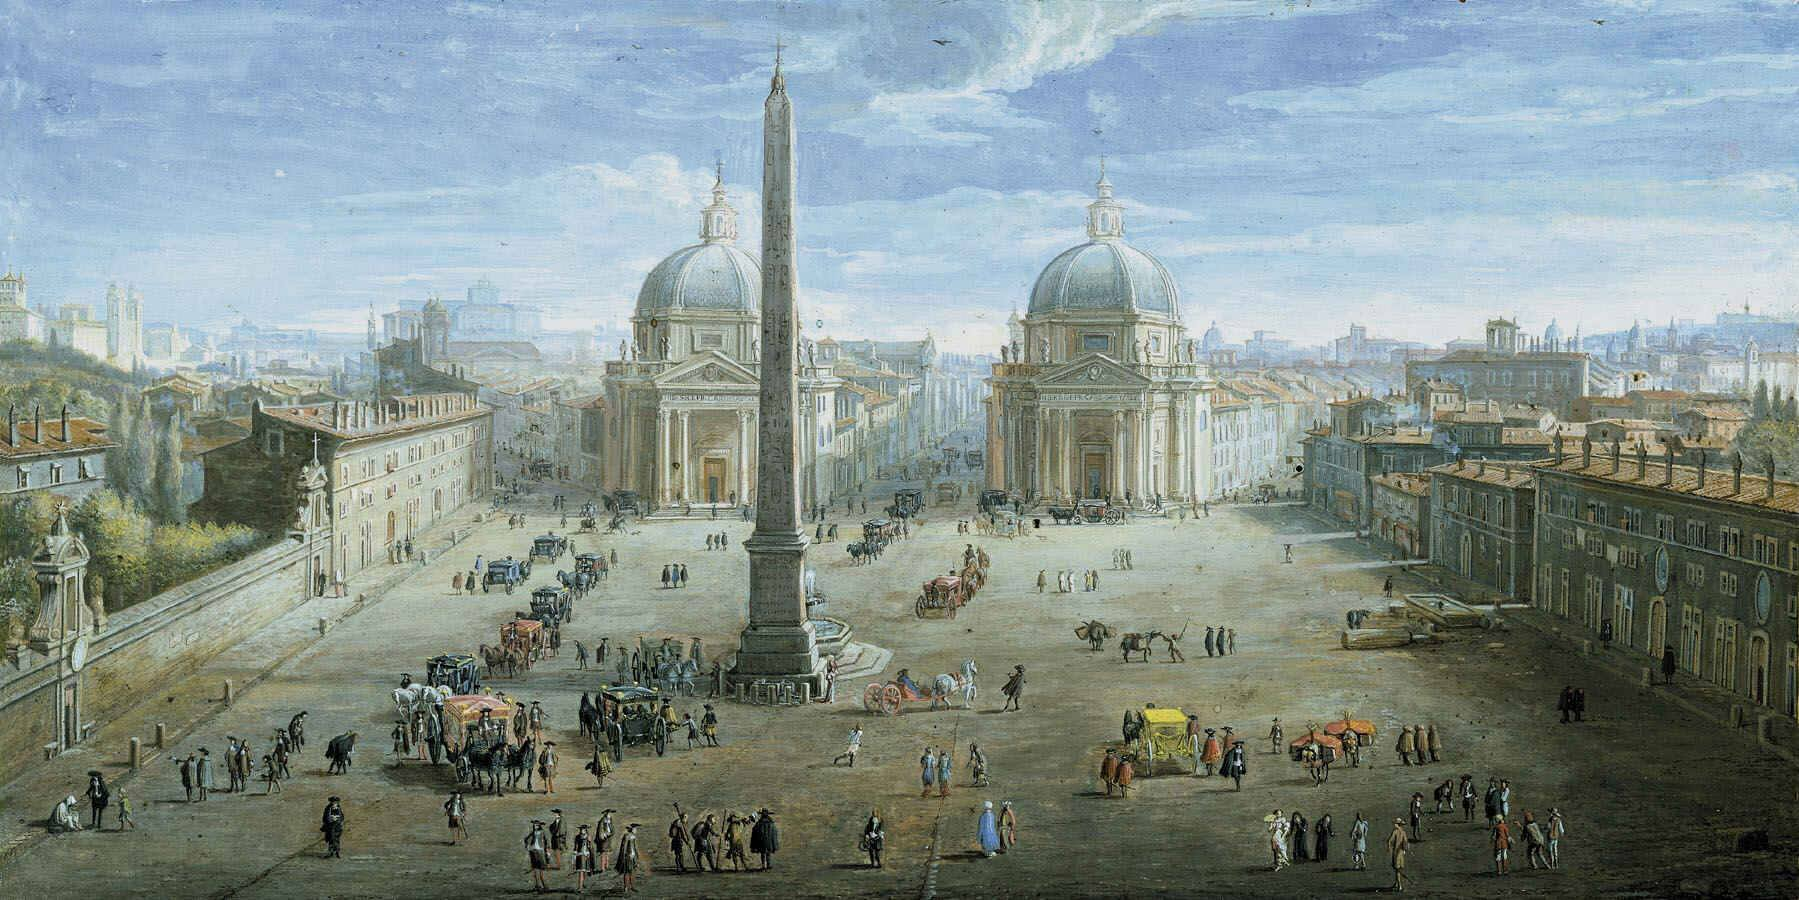
\includegraphics[width=1\textwidth]{/Users/Pancratii/GitHub/phd/Sections/Projeto_de_Pesquisa_2023-03-18_Teste/Pictures/popolo.jpeg} 
	            \captionsetup{labelfont=bf}
	            \caption{Vista da \textit{Piazza del Popolo}, em Roma, por Caspar Van Wittel (1652–1736). \textbf{Fonte:} Wikimedia Commons / Sotherby's (coleção privada).}
	            \label{fig:popolo}
            \end{figure}   

            Discorramos rapidamente sobre a ideia de \textit{forma} e traçado. Traçado é o particípio do verbo traçar, \textit{i.e.,} desenhar traços, riscar, sendo o ato ou efeito desse mesmo verbo, resultando, portando, em um `conjunto de traços', ou, no nosso caso, no `desenho que representa uma estrutura arquitetônica ou urbanística', o que é equivalente a dizer `planta', `projeto', ou, para usar um termo mais antigo, `traça' (PRIBERAM, TRAÇADO, 2023). Na língua rústica do latim, `tracto' que dizer `traçar sulcos', e `tractus' é a `delimitação por meio de traços; região, lugar, quarteirão' (FARIA, 1962, p. 1010). Penso que não haja melhor definição que essa: `delimitação por meio de traços' – que corrobora com a ideia de trajetória de estrada ou mesmo linha férrea (PRIBERAM, TRAÇADO, 2023). \textit{Forma,} porém, é um termo mais complexo.

            \begin{figure}
	            \centering
	            \includegraphics[width=1\textwidth]{/Users/Pancratii/GitHub/phd/Sections/Projeto_de_Pesquisa_2023-03-18_Teste/Pictures/nolli_popolo.png}
	            \captionsetup{labelfont=bf}
	            \caption{\textit{La nuova topografia di Roma} (detalhe), de Gianbattista Nolli (1701-1756), com a \textit{Piazza del Popolo} ao norte. \textbf{Fonte:} UC Berkeley Library.}
	            \label{fig:nolli_popolo}
            \end{figure} 

            \textit{Forma} é a `configuração das coisas na parte exterior', o que é equivalente a `feitio' e `formato' (PRIMERAM, FORMA, 2023). No latim, a coisa complica um pouco, com \textit{`forma'} querendo dizer `fôrma' (que em português é um `molde sobre o qual ou dentro do qual se coloca alguma substância fluida, que toma o feitio desse molde'), ou `todo objeto feito na fôrma'; pode, de fato, ser entendida como `desenho, modelo, planta', mas também pode ser entendida como `tipo ideal', ou ainda como `conformação, configuração, constituição' (FARIA, 1962, p. 407). E, se formos para o campo da filosofia, aí é que a confusão aumenta, pois temos um `sentido filosófico e particularmente metafísico', um `sentido lógico', outro `epistemológico', um metodológico', e, por fim, ainda um `sentido estético' (MORA, 2001b, p. 1126) – e, portanto, a ideia de \textit{`forma'} escapa-nos neste momento.

            Desse modo, na presente pesquisa, meu foco se direciona ao `traçado urbano' e não à \textit{`forma} urbana'. No entanto, é necessário esclarecer que o termo `traçado urbano', por sua vez, pode ter mais de uma acepção. Se pensarmos que a \textit{`forma'} da cidade é constituída por seu aspecto tridimensional,
                \footnote[6]{Aqui faço minhas as palavras de José Lamas (2010, pp. 41 e 48), ao dizer que a forma urbana corresponde "ao meio urbano como arquitectura, ou seja, um conjunto de objectos arquitectónicos ligados entre si por relações espaciais" e que é "a materialização no espaço da resposta a um contexto preciso".} 
            com suas edificações e demais estruturas, podemos deduzir que o `traçado' é a marca deixada no solo por essa \textit{`forma'}. Logo, o `traçado' da cidade seria o sulco resultante dos limites dos lotes e quarteirões e dos contornos edificados (que, não raro, definem o próprio desenho das vias, por meio da conjunção de fachadas).
                \footnote[7]{Note-se que, diferente do que atualmente é lugar comum, o que definia o que era ou não a rua, seu limite, seu contorno, seu espaço, era precisamente a fachada da edificação, que imprime essa linha ao mesmo tempo imaginária e real no solo, diferente do que ocorre hoje. Hoje, o lugar comum é aquele de que o que define a via é o meio-fio — ou o limite do lote, que não coincide com a implantação da edificação, com a marca que a mesma deixa sobre o solo. E isso é fruto da desvinculação entre edificação e lote, entre os limites da edificação e os limites do lote. Mas, se olharmos para nosso passado urbano, veremos algo bem diferente. Basta olharmos uma pintura de Caspar Van Wittel da \textit{Piazza Navona} em Roma e veremos como a praça já era muitíssimo bem definida (pelas edificações), mesmo sem qualquer indício de calçamento, e muito menos de meio-fio.} 

            No entanto, aqui, pretendo que o termo `traçado urbano' tome uma ênfase particular. Isso não exclui o sentido aludido acima, posto que tratarei de contornos edificados, lotes e quarteirões ao falar de `traçado urbano' ao longo desta tese – porém serei específico quando o fizer. Desse modo, a ênfase que quero dar é a de `traçado urbano' enquanto sinônimo de `espaço público', tanto na definição de Vitor Oliveira (2016)
                \footnote[8]{\textit{`The public spaces system of a city includes (...) the open spaces for movement, which we designate, in a simplified way, as streets, (...) [and] also the open spaces for permanence, which we designate as squares and gardens.'} (OLIVEIRA, 2016, p. 17).} 
            quanto, particularmente, na visão de Huimin Ji e Wowo Ding (2021) – que trazem uma releitura contemporânea de Gianbattista Nolli (\autoref{fig:nolli_popolo}). Assim, o termo `traçado urbano' se relaciona com as vias, praças e áreas públicas de edificações – espaços com acesso franqueado ao público. Percursos, nós e polos abertos e fechados, cobertos e descobertos, percorríveis em um único plano contínuo: o plano do solo.
                \footnote[9]{Podemos chamar esse plano de `térreo', ainda que ele comporte variações de altitude e inclinação; porém a ideia é a de que esse é o "plano-base" da cidade, a partir do qual se desenvolvem as edificações, para cima ou para baixo.} 
            Por vias podemos tomar percursos como ruas, calçadões, \textit{woonerfs}, escadarias e alamedas e espaços abertos de parques urbanos (excluídos os maciços vegetais), levando em conta a apropriação dos elementos contidos nesses espaços, como ocorre com os canteiros (HANNES, 2016);
                \footnote[10]{Canteiros que, atualmente, são considerados algo à parte, algo que não é inerente à via, mas que a define e delimita, posto que, para boa parte das prefeituras, o que determina o limite da via não é o \textit{continuum} das fachadas das edificações, senão o limite dos lotes (muros), as guias de meio-fio e os canteiros: elementos definidores da rua que não mais estão destinados a um uso comum.} 
            bem como estacionamentos descobertos, além de rodovias e ferrovias (posto que servem de passagem para pessoas e suas mercadorias e que possuem uma marca sobre o solo que se relaciona com o desenho do restante da cidade). Por praças, podemos entender tanto a clássica praça, espaço aberto de dimensões superiores à da rua, o largo, o \textit{pocket park}, desde que descobertos – exceção feita aos \textit{`annodamenti'} (dos quais se tratará no momento oportuno), que ficam em uma situação ambígua de área pública de edificação e praça. E as áreas públicas de edificações podem ser exemplificadas pelas naves das igrejas, pelas platéias dos teatros e pelos halls, corredores, pátios e praças cobertas dos  edifícios públicos, galerias comerciais, mercados e \textit{shopping centers}.

            Dito isso, reforço que: em relação às `formas' edificadas, conhecemos os motivos da crise atual  – e podemos mesmo ir mais a fundo, entendendo as dinâmicas inerentes aos materiais, à economia, às tendências ditadas de tempos em tempos pelas publicações e sua relação com o design de outras áreas. Temos ideia de como estabelecer um liame com o passado, inclusive com exemplos projetuais – e, quando não (como no caso do Brasil), temos um método para `ler' as pré-existências edificadas e, a partir delas, deduzir o \textit{tipo} edilício de um território, de modo a ter o balizador para novas edificações. E nisso reside a força da escola italiana de tipomorfologia urbana. Todavia, mais uma vez: se podemos sabemos como obter respostas em relação à \textit{forma} da cidade, o mesmo não se dá em relação ao seu traçado.

            \section{Rendimento}%conteúdo anterior [reprovado 10 OUT 2023]
            
            \textit{Rendimento}, ``grau de coerência [de algo] com o contexto'' (Maffei, 2003, p. 82, tradução nossa).  Até minha dissertação, pude levantar duas acepções para o termo: uma, o \textit{`rendimento} edilício', e outra, o \textit{`rendimento'} territorial. A primeira é uma dialética entre a ação do homem e uma reação do ambiente (antrópico) no qual ele está inserido (Caniggia e Maffei, 2008, p. 52). A segunda é a medida com que um território pode ser utilizado pelo homem (Carlotti, 1995, p. 19). Dessas duas escalas, pude deduzir uma nova acepção, que intitulei \textit{`rendimento} urbano', ou seja, ``a coerência intrínseca entre o traçado da forma urbana e o contexto natural'' (Costa, 2020, p. 52). Assim, tomando esse ponto de partida, faz-se necessário destrinchar alguns conceitos e definições.

            A proposição inicial da minha tese é a de que `é possível projetar traçados urbanos morfologicamente adequados ao contexto'. Mais que isso, tais traçados não são traçados `adaptados', com uma forma concebida \textit{a priori}, que só depois é confrontada com a realidade e então deformada por ela – como o seria um \textit{grid}, uma matriz de linhas ortogonais. Ao contrário, tais traçados devem ser adequados ao contexto desde sua concepção. Ou seja, o contexto vem antes. É ele que direciona o projeto. Ou melhor, o processo de projeto parte da consideração de suas formas, e, desse modo, o contexto dá a \textit{forma} do traçado urbano. Nesse sentido, vale a pena esmiuçar melhor o que quero dizer com termos como `forma', `traçado', `contexto', `morfologicamente adequado', e outros termos relacionados como `território' e `paisagem' – quero dizer, é necessário mostrar suas acepções e de quais autores extraio tais conceitos.

            \section{Traçado urbano}%conteúdo anterior [reprovado 10 OUT 2023]
                \subsection{Forma urbana}
                \subsection{Elementos antrópicos do traçado: percursos, nós e polos}
                \subsection{Estruturas naturais subjacentes ao traçado}
                    \subsubsection*{Definições de paisagem e território}
                Para Giuseppe Strappa (2014, p. 19, tradução nossa), %https://issuu.com/giuseppestrappa/docs/strappa_diadi_mediterranee_2014
                    ``o território é um modo de olhar o mundo (...), [de ler] a forma das coisas (dos solos, dos percursos, dos assentamentos) para compreender sua estrutura, entender suas origens [e] possíveis transformações''. O território, continua, ``é o conjunto inscindível de solo e trabalho do homem que o habita e transforma, [em suma,] é arquitetura.'' O termo `paisagem', portanto, ``é o aspecto reconhecível da sua estrutura, a sua forma [, que contém um conjunto de contribuições].'' Ou seja, a `paisagem' para Strappa é a forma do território. Um não contém o outro, mas um é a manifestação do outro.\footnote[11]{\textit{``In architettura il territorio è un modo di guardare il mondo. Di leggere, cioè, la forma delle cose (dei suoli, dei percorsi, degli insediamenti) per afferrarne la struttura, capirne le origini, le possibili trasformazioni. Il territorio è l'insieme inscindibile di suolo e lavoro dell'uomo che lo abita e lo trasforma, è architettura. Il termine `paesaggio' è l'aspetto riconoscibile della sua struttura, la sua forma che contiene un insieme di contributi''} (Strappa, 2014, p. 19).}

                    Em uma nota de rodapé, Strappa (2019, \textit{s.p.}) escreve ainda: %http://www.giuseppestrappa.it/wp-content/uploads/2019/10/cap.-10-territorio-per-il-corso.pdf http://www.giuseppestrappa.it/?p=8355
                    \begin{quotation}
                        ``\emph{Land-scape} significa em inglês `modelagem da terra', com ênfase no aspecto natural do ambiente cognitivo com o qual o termo está associado. Ele se opõe ao termo italiano \emph{`paesaggio'} (francês \emph{`paysage'}, espanhol \emph{`paisaje'}), associado ao termo \emph{`paese'} e, portanto, ao latim \emph{`pagus'}, que significa vila, reconhecendo, de maneira concisa, uma relação de solidariedade entre a terra e o assentamento humano. Portanto, a paisagem como expressão cultural está ligada ao espaço habitado, à cooperação entre recursos naturais e artificiais, às transformações que interpretam a forma de picos orográficos, vales, planícies e sua capacidade de se tornar um ambiente construído. Em resumo, [paisagem] é o aspecto visível do território, a expressão concisa de sua estrutura'' (tradução nossa).\footnote[12]{\textit{``Land-scape'' means in English ``modelling of the earth'', with an emphasis on the natural aspect of the cognitive environment the term is associated with. It is opposed to the Italian term ``paesaggio'' (French ``paysage'', Spanish ``paisaje'') associated with the term ``paese'' and hence to the Latin ``pagus'' meaning village, acknowledging, in a concise manner, a relationship of solidarity between the land and human settlement.Therefore, the landscape as a cultural expression is linked to the inhabited space, to the cooperation between natural and artificial resources, to the transformations that interpret the form of orographic peaks, valleys, plains and their ability to become a built environment. In short, it is the territory’s visible aspect, the concise expression of its structure''} (Strappa, 2019, \textit{s.p.}).}
                    \end{quotation}

                \subsection{Relações entre traçado urbano, parcelamento rural e áreas não-antropizadas}
                
                Não é possível reconhecer o traçado urbano como um mero objeto autônomo, sem relação com o solo sobre o qual se assenta, solo esse que também é subjacente ao território que circunda esse traçado. Desse modo, o traçado urbano deve ser entendido dentro do \textit{framework} dado pelo território, ambos sustentados por um solo com características naturais peculiares a cada lugar, formando, assim, uma paisagem só.\footnote[13]{Para Strappa (2013, \textit{s.p.}), a noção de território deriva do nexo entre a ideia de contexto natural e transformações antrópicas desse mesmo contexto natural, o que o faz entender a paisagem como aspecto visível de uma estrutura de relações que conecta os diversos graus e escalas do universo construído dentro da noção de organismo. Escreve: \textit{``Il concetto di territorio deriva dal nesso che lega l’idea di suolo naturale a quella delle trasformazioni artificiali operate dall’uomo nel processo di antropizzazione (trasformazione abitativa e produttiva) del suolo stesso. Noi cogliamo questo processo attraverso momentanei stati di equilibrio che  restituiscono un’idea discreta di una sequenza storica che è, invece, flusso continuo di modificazioni e rivolgimenti.
                Per questo non è comprensibile il senso storico-processuale di un organismo urbano o di un sistema di percorrenze, se non si colloca la loro formazione all’interno di un rapporto di necessità con l’insieme delle relazioni instaurate nel tempo e nello spazio entro il proprio intorno territoriale. Questa forma del territorio antropizzato non é che l’aspetto visibile di una struttura di relazioni che lega nella nozione di organismo i diversi gradi scalari del costruito e che indicheremo col termine `paesaggio'.''} Essa definição mesma de `paisagem' serve para indicar o que é o contexto antrópico.}

            \section{\textit{Modus faciendi} atual}
                \subsection{Manuais, guias e leis de parcelamento do solo}
                \subsection{Entrevistas sobre princípios que norteiam o desenho dos traçados}
                \subsection{Rendimento econômico}
            \section{Morfoadequabilidade: uma nova definição} %Ver se não fica melhor antes da seção sobre o modus faciendi atual.

        
        \chapter[A escolha de uma solução]{artefato a desenvolver}

\end{document}
